% Saberes básicos (LOMLOE) asociados a esta unidad
%
% D. La interacción
%   - Predicción de movimientos sencillos a partir de los conceptos de la cinemática, formulando
%     hipótesis comprobables sobre valores futuros de estas magnitudes, validándolas a través del
%     cálculo numérico, la interpretación de gráficas o el trabajo experimental:
%     toda la unidad trabaja posición, distancia, desplazamiento, velocidad y aceleración,
%     tanto a partir de tablas y gráficas posición-tiempo/velocidad-tiempo (MRU y MRUA) como
%     mediante cálculo numérico en ejemplos y ejercicios resueltos.
%   (Las fuerzas, las leyes de Newton y el peso están en la Unidad 8, Forces.)
%
% A. Las destrezas científicas básicas
%   - Unidades del Sistema Internacional y herramientas matemáticas: uso sistemático de \unit{}
%     y \qty{} (m/s, m/s^2), factores de conversión entre unidades de velocidad, y
%     construcción/interpretación de tablas y gráficas para representar y predecir el movimiento.
%
% (Los bloques B -materia-, C -energía- y E -el cambio- no son objeto de esta unidad.)

\spacing{1.3}
\raggedbottom % pages with large figures end where the text ends (no stretched gaps between boxes)

\section{Introduction}

Everything around us moves: cars on the road, a ball in the playground, the blood in our veins, the Earth around the Sun\ldots{} Even when you are sitting still in class, you are moving together with the Earth! The part of physics that studies motion is called \negsubro{kinematics}.

\begin{definition}[Kinematics]
    The part of physics that studies the \textbf{motion} of bodies: how they move, how fast and in which direction, \textbf{without} studying the causes of that motion (the forces).
\end{definition}

\begin{definition}[Motion]
    A body is in \textbf{motion} when its \textbf{position changes} over time with respect to another body that we take as a reference. If its position does not change, the body is \textbf{at rest}.
\end{definition}

In this unit we will learn to describe motion using quantities such as \textbf{position}, \textbf{displacement}, \textbf{velocity} and \textbf{acceleration}; and we will study two simple types of motion (uniform motion and uniformly accelerated motion) using tables, graphs and formulas. In the next unit, \textbf{Forces}, we will see with \textbf{Newton's laws} how forces change the motion of bodies.

%----------------------------------------------------------------------------------------

\section{Quantities describing motion}

To describe a motion we need some basic quantities. Let us see them one by one:

\begin{enumerate}[label=\numberballmDarkTeal]
    \item \negsubro{Frame of reference}.
    \begin{definition}[Frame of reference]
        A point, or set of points, that we consider to be fixed, and use to describe the position and motion of other bodies.
    \end{definition}
    \begin{impt}
        \negsubro{Motion is relative}. Whether a body is moving or not depends on the frame of reference we choose: a body \textbf{moves} if its position changes with respect to the frame of reference, and the same body can be in motion with respect to one frame of reference and at rest with respect to another.
    \end{impt}
    \begin{figure}[H]
        \centering
        % [FIGURA ORIGINAL] \includegraphics[width=\textwidth]{Unit_7/reference_frame}
        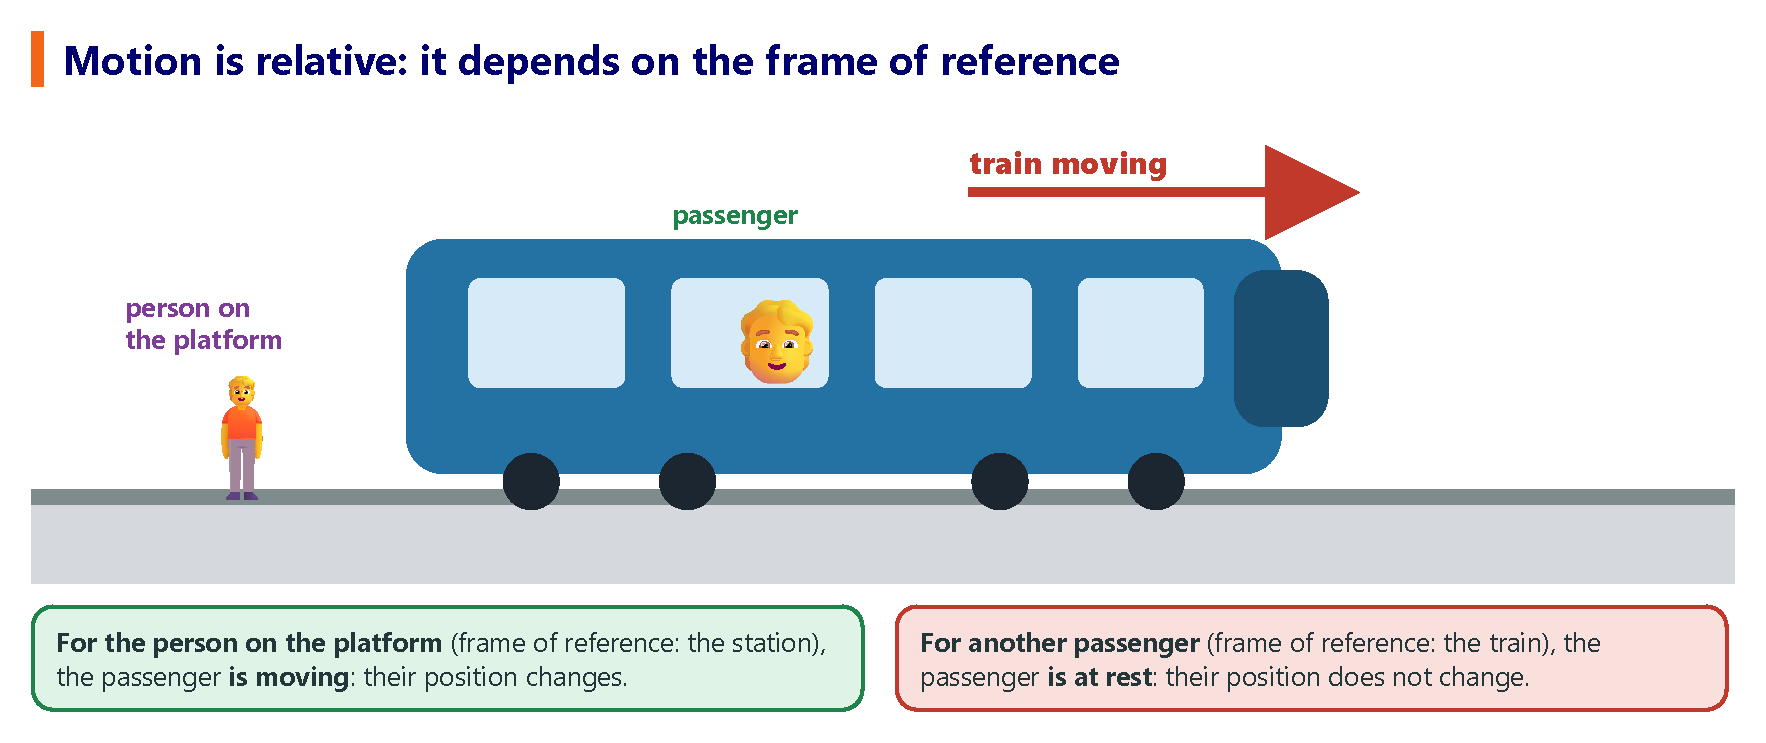
\includegraphics[width=\textwidth]{FigurasSVG/Unit_7_Motion/pdf/reference_frame.pdf}
        \caption{Whether the passenger moves or not depends on the frame of reference.}
        \label{fig:u7_reference_frame}
    \end{figure}

    \item \negsubro{Trajectory}.
    \begin{definition}[Trajectory]
        The line that a moving object follows. It can be \textbf{rectilinear} (straight), \textbf{circular}, \textbf{parabolic}, or any other shape.
    \end{definition}

    \item \negsubro{Position}.
    \begin{definition}[Position]
        The place occupied by a moving object at a given moment, measured from the origin of the frame of reference. It is represented by the letter \(x\).
    \end{definition}
    The position \(x\) tells us \textbf{how far} the object is from the origin, so it is a quantity of \textbf{length}: in the SI it is measured in \textbf{metres} (\unit{\m}). We write \(x_i\) for the \textbf{initial} position and \(x_f\) for the \textbf{final} position.

    \item \negsubro{Distance travelled}.
    \begin{definition}[Distance travelled]
        The length of the trajectory (path) followed by the moving object.
    \end{definition}

    \item \negsubro{Displacement}.
    \begin{definition}[Displacement]
        The change in position of a moving object: its final position minus its initial position. It is the straight-line distance between the initial and the final position.
        \begin{equation*}
            \Delta x = x_f - x_i
        \end{equation*}
    \end{definition}
    \begin{itemize}
        \item The symbol \(\Delta\) (the Greek letter \textbf{delta}) means ``\textbf{change in}'': \(\Delta x\) is read ``delta x'' and means ``change in position''.
        \item \(x_f\) is the \textbf{final} position and \(x_i\) the \textbf{initial} position. Both are positions, so \(\Delta x\) is also a \textbf{length} and is measured in \textbf{metres}.
        \item If \(\Delta x\) is \textbf{positive}, the object has moved away from the origin (in the positive direction); if it is \textbf{negative}, it has moved in the opposite direction.
    \end{itemize}
    \begin{figure}[H]
        \centering
        % [FIGURA ORIGINAL] \includegraphics[width=\textwidth]{Unit_7/delta_x_t}
        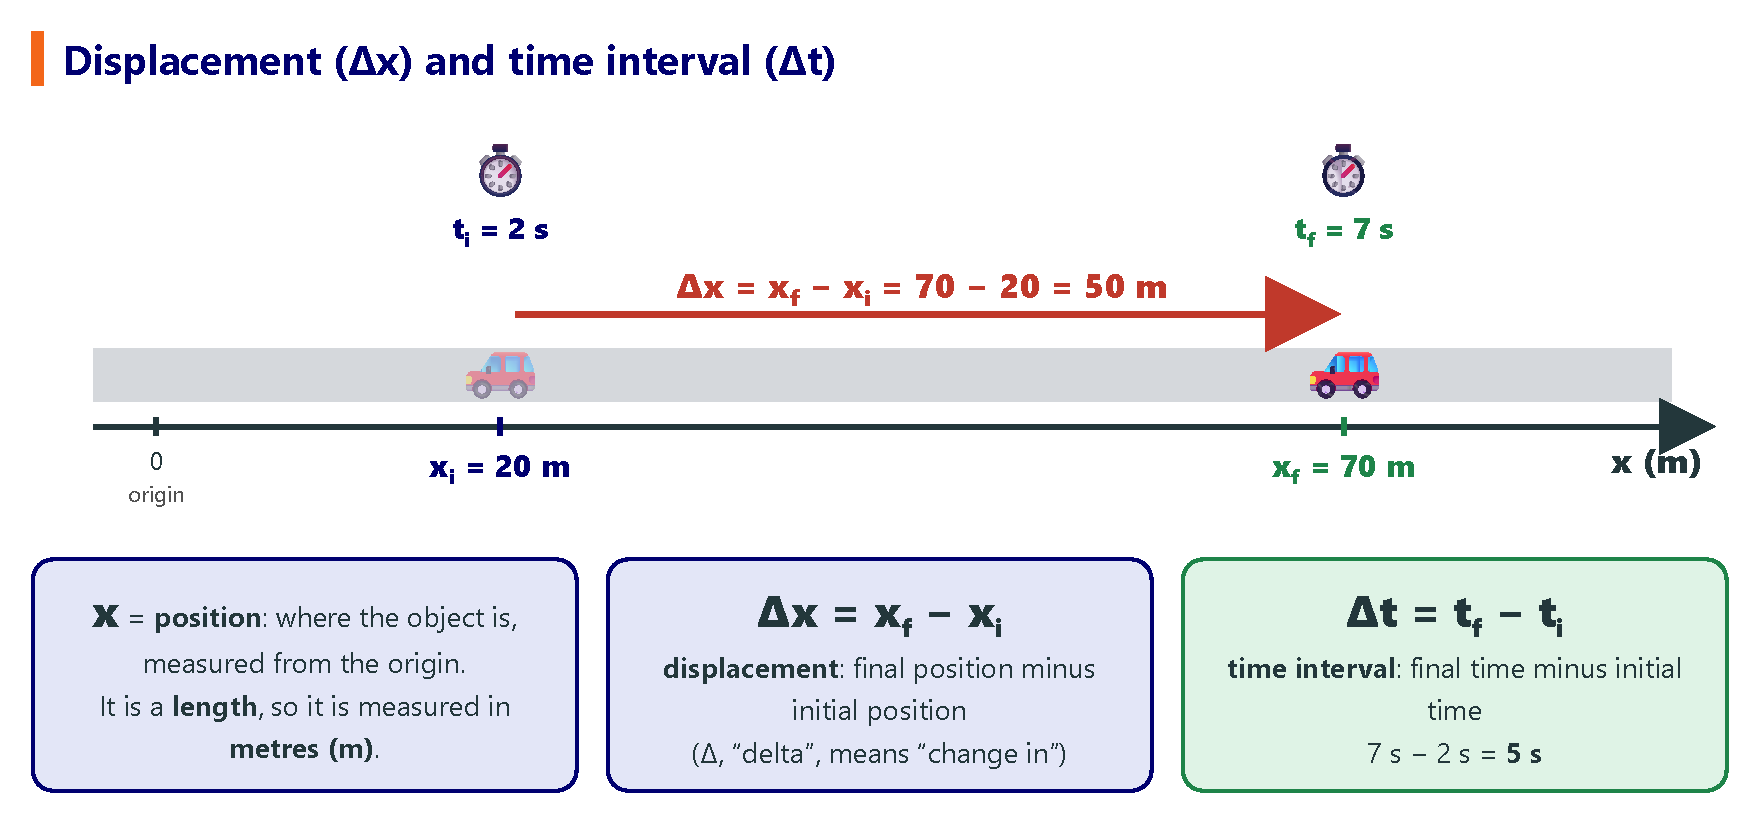
\includegraphics[width=\textwidth]{FigurasSVG/Unit_7_Motion/pdf/delta_x_t.pdf}
        \caption{The displacement is the final position minus the initial position; the time interval is the final time minus the initial time.}
        \label{fig:u7_delta_x_t}
    \end{figure}
    \begin{figure}[H]
        \centering
        % [FIGURA ORIGINAL] \includegraphics[width=\textwidth]{Unit_7/distance_displacement}
        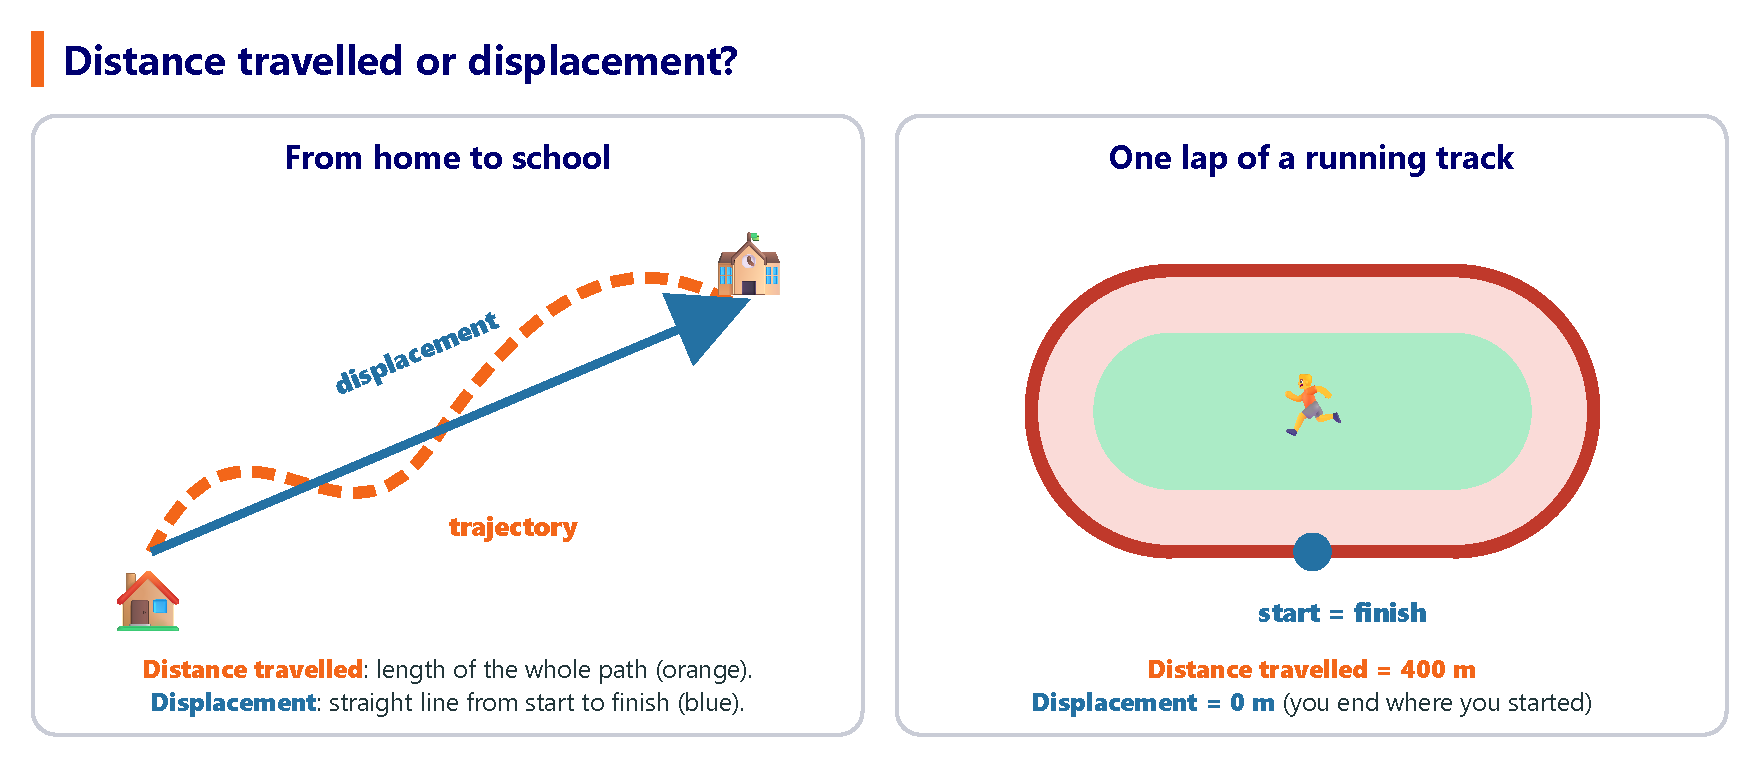
\includegraphics[width=\textwidth]{FigurasSVG/Unit_7_Motion/pdf/distance_displacement.pdf}
        \caption{Distance travelled (the whole path) and displacement (the straight line from start to finish).}
        \label{fig:u7_distance_displacement}
    \end{figure}
\end{enumerate}

\begin{example}
    \textbf{A car is at \(x_i = \qty{20}{\m}\) and, after a while, it is at \(x_f = \qty{70}{\m}\). Calculate its displacement.}
    \begin{equation*}
        \Delta x = x_f - x_i = \qty{70}{\m} - \qty{20}{\m} = \textcolor{red}{\qty{50}{\m}}
    \end{equation*}
\end{example}

\begin{exercise}
    A runner does one full lap of a \qty{400}{\m} circular track, starting and finishing at the same point.
    \begin{enumerate}[label=\letraminuscula]
        \item What distance has the runner travelled?
        \item What is the runner's displacement?
    \end{enumerate}
    \begin{solu}
        \begin{enumerate}[label=\alph*)]
            \item Distance travelled \(= \qty{400}{\m}\) (the length of the whole lap).
            \item Displacement \(= \qty{0}{\m}\), because the initial and final positions are the same point.
        \end{enumerate}
    \end{solu}
\end{exercise}

\begin{exercise}
    Two friends are sitting on parallel, stationary buses. Suddenly, one of the buses starts moving.
    \begin{enumerate}[label=\letraminuscula]
        \item Explain why, at first, it is difficult to tell which bus is moving.
        \item If you take the other bus as your frame of reference, can you tell which one is moving?
    \end{enumerate}
    \begin{solu}
        \begin{enumerate}[label=\alph*)]
            \item Motion is relative: from inside each bus, all you can perceive at first is the relative movement between the two buses, so it looks the same whichever one is actually moving.
            \item Yes: if you take the other bus as the fixed frame of reference, you can tell that \emph{your} bus is moving with respect to it as soon as the distance between the two buses changes.
        \end{enumerate}
    \end{solu}
\end{exercise}

\begin{exercise}
    A cyclist rides \qty{300}{\m} north along a straight road, then turns around and rides back \qty{120}{\m} south.
    \begin{enumerate}[label=\letraminuscula]
        \item Calculate the distance travelled.
        \item Calculate the displacement.
    \end{enumerate}
    \begin{solu}
        \begin{enumerate}[label=\alph*)]
            \item Distance travelled \(= \qty{300}{\m} + \qty{120}{\m} = \qty{420}{\m}\) (we add up every metre covered, regardless of direction).
            \item Displacement \(= \qty{300}{\m} - \qty{120}{\m} = \qty{180}{\m}\) north (the straight-line distance between the starting point and the final point).
        \end{enumerate}
    \end{solu}
\end{exercise}

\begin{exercise}
    A hiker walks \qty{2}{\km} east along a straight path, then turns around and walks \qty{5}{\km} west.
    \begin{enumerate}[label=\letraminuscula]
        \item Calculate the distance travelled.
        \item Calculate the displacement.
    \end{enumerate}
    \begin{solu}
        \begin{enumerate}[label=\alph*)]
            \item Distance travelled \(= \qty{2}{\km} + \qty{5}{\km} = \qty{7}{\km}\).
            \item Displacement \(= \qty{5}{\km} - \qty{2}{\km} = \qty{3}{\km}\) west (the straight-line distance from the start to the final point, in the direction of the larger leg).
        \end{enumerate}
    \end{solu}
\end{exercise}

%----------------------------------------------------------------------------------------

\section{Velocity}

\begin{definition}[Velocity]
    A quantity that measures how fast an object changes its position. It is represented by the letter \(v\), and it is the \textbf{displacement} divided by the \textbf{time interval}:
    \begin{equation*}
        v = \dfrac{\Delta x}{\Delta t} = \dfrac{x_f - x_i}{t_f - t_i}
    \end{equation*}
    In the SI, velocity is measured in \unit{\mps}.
\end{definition}

\begin{itemize}
    \item \(\Delta x = x_f - x_i\) is the \textbf{displacement} (final position minus initial position), in metres.
    \item \(\Delta t = t_f - t_i\) is the \textbf{time interval}: the \textbf{final} time \(t_f\) minus the \textbf{initial} time \(t_i\), in seconds.
\end{itemize}

\begin{impt}
    \negsubro{When nothing else is said}: if the exercise does not give the initial position or the initial time, we take
    \begin{equation*}
        x_i = \qty{0}{\m} \qquad\text{and}\qquad t_i = \qty{0}{\s}
    \end{equation*}
    Then \(\Delta x = x_f - 0 = x_f\) and \(\Delta t = t_f - 0 = t_f\). We simply write \(x_f\) as \(x\) and \(t_f\) as \(t\), and the formula of velocity becomes:
    \begin{equation*}
        v = \dfrac{x}{t}
    \end{equation*}
\end{impt}

\begin{example}
    \textbf{A car is at \(x_i = \qty{20}{\m}\) when the stopwatch reads \(t_i = \qty{2}{\s}\), and at \(x_f = \qty{70}{\m}\) when it reads \(t_f = \qty{7}{\s}\). Calculate its velocity.}
    \begin{equation*}
        v = \dfrac{x_f - x_i}{t_f - t_i} = \dfrac{\qty{70}{\m} - \qty{20}{\m}}{\qty{7}{\s} - \qty{2}{\s}} = \dfrac{\qty{50}{\m}}{\qty{5}{\s}} = \textcolor{red}{\qty{10}{\mps}}
    \end{equation*}
\end{example}

\begin{example}
    \textbf{A runner covers \qty{100}{\m} in \qty{12.5}{\s}. Calculate her velocity.} Nothing is said about the start, so \(x_i = \qty{0}{\m}\) and \(t_i = \qty{0}{\s}\):
    \begin{equation*}
        v = \dfrac{x}{t} = \dfrac{\qty{100}{\m}}{\qty{12.5}{\s}} = \textcolor{red}{\qty{8}{\mps}}
    \end{equation*}
\end{example}

In everyday language we often say \textbf{speed} for how fast something moves. Other common units are \unit{\kmph}, m/min, miles per hour or knots. To compare speeds given in different units, we must first convert them to the \textbf{same} unit, using conversion factors.

\begin{figure}[H]
    \centering
    % [FIGURA ORIGINAL] \includegraphics[width=\textwidth]{Unit_7/speeds}
    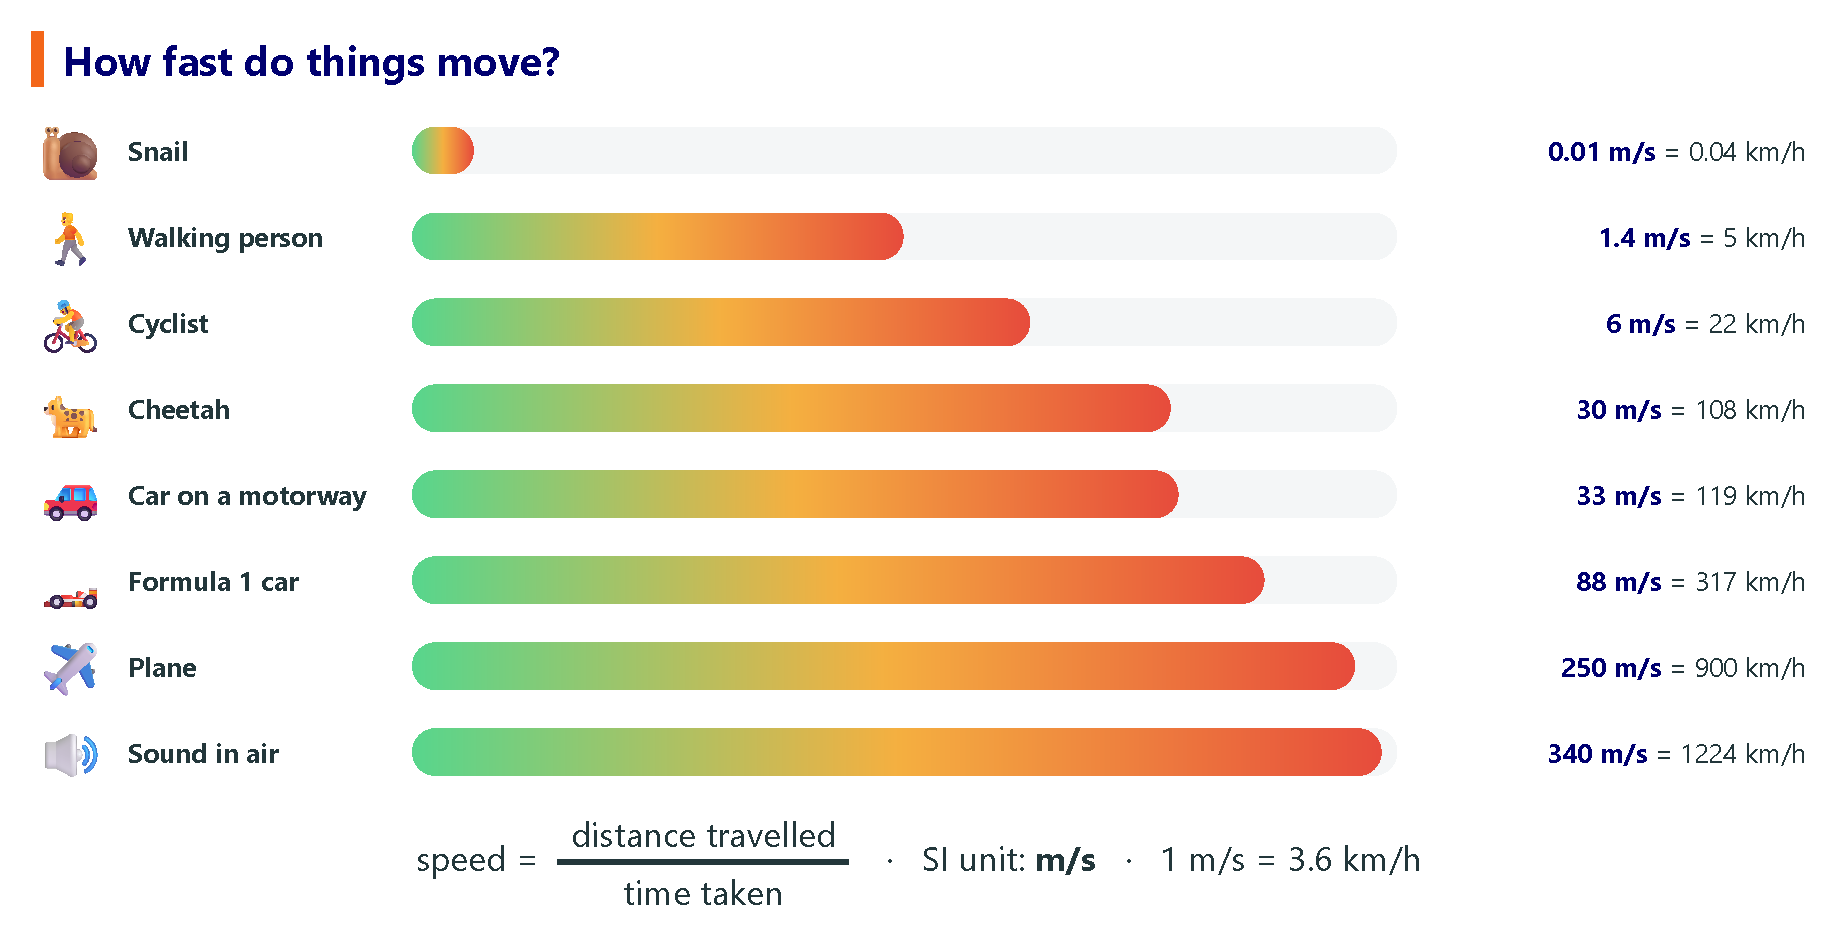
\includegraphics[width=\textwidth]{FigurasSVG/Unit_7_Motion/pdf/speeds.pdf}
    \caption{Speeds of some animals, vehicles and sound, in m/s and km/h.}
    \label{fig:u7_speeds}
\end{figure}

\begin{didyouknow}
    Even when you are sitting still in class, you are travelling at about \qty{107000}{\kmph}! That is the speed of the Earth in its orbit around the Sun. Motion really is relative.
\end{didyouknow}

\begin{example}
    \textbf{A car is travelling at \qty{90}{\kmph} and a motorbike at \qty{30}{\mps}. Which one is moving faster?}
    \begin{equation*}
        90 \dfrac{\text{km}}{\text{h}} \cdot \dfrac{\qty{1000}{\m}}{\qty{1}{\km}} \cdot \dfrac{\qty{1}{\hour}}{\qty{3600}{\s}} = \qty{25}{\mps}
    \end{equation*}
    Since \qty{30}{\mps} \(>\) \qty{25}{\mps}, \textbf{the motorbike is moving faster}.
\end{example}

\subsection{Average velocity and instantaneous velocity}

\begin{itemize}
    \item \negsubro{Average velocity}: the total distance travelled divided by the total time taken for a whole journey.
    \item \negsubro{Instantaneous velocity}: the velocity of a moving object at one specific moment, read on a speedometer.
\end{itemize}

\begin{impt}
    A moving object's velocity is usually \textbf{not} constant throughout a journey, so its average velocity is generally different from its instantaneous velocity at any given moment. They can only be the same if the object moves at a constant velocity for the whole journey.
\end{impt}

\begin{example}
    \textbf{A bus covers \qty{1500}{\m} in \qty{150}{\s}. Calculate its average velocity.}
    \begin{equation*}
        v_{\text{average}} = \dfrac{x}{t} = \dfrac{\qty{1500}{\m}}{\qty{150}{\s}} = \qty{10}{\mps} = \qty{36}{\kmph}
    \end{equation*}
\end{example}

\begin{exercise}
    Which animal is travelling faster: a centipede at \qty{40}{\cm\per\s}, or a tortoise at \qty{16.8}{\m\per\minute}?
    \begin{solu}
        Convert both to the same unit, \unit{\cm\per\s}: \\
        Tortoise: \(16.8 \dfrac{\text{m}}{\text{min}} \cdot \dfrac{\qty{100}{\cm}}{\qty{1}{\m}} \cdot \dfrac{\qty{1}{\minute}}{\qty{60}{\s}} = \qty{28}{\cm\per\s}\). \\
        Since \qty{40}{\cm\per\s} \(>\) \qty{28}{\cm\per\s}, \textbf{the centipede is faster}.
    \end{solu}
\end{exercise}

\begin{exercise}
    A commercial plane's cruising speed is \qty{900}{\kmph}. The maximum speed reached in a Formula 1 race was \qty{88}{\mps}. Which is higher?
    \begin{solu}
        Convert the plane's speed to \unit{\mps}: \(900 \dfrac{\text{km}}{\text{h}} \cdot \dfrac{\qty{1000}{\m}}{\qty{1}{\km}} \cdot \dfrac{\qty{1}{\hour}}{\qty{3600}{\s}} = \qty{250}{\mps}\). \\
        Since \qty{250}{\mps} \(>\) \qty{88}{\mps}, \textbf{the plane's cruising speed is higher}.
    \end{solu}
\end{exercise}

\begin{exercise}
    A lorry driver covers the \qty{300}{\km} between two cities. For the first \qty{200}{\km} she drives at an average speed of \qty{100}{\kmph}, and for the remaining \qty{100}{\km}, due to traffic, her average speed drops to \qty{50}{\kmph}.
    \begin{enumerate}[label=\letraminuscula]
        \item Calculate the time taken for each part of the journey.
        \item Calculate the average speed for the whole journey. Is it the mean of \qty{100}{\kmph} and \qty{50}{\kmph}? Explain why, or why not.
    \end{enumerate}
    \begin{solu}
        \begin{enumerate}[label=\alph*)]
            \item \(t_1 = \dfrac{\qty{200}{\km}}{\qty{100}{\kmph}} = \qty{2}{\hour}\); \quad \(t_2 = \dfrac{\qty{100}{\km}}{\qty{50}{\kmph}} = \qty{2}{\hour}\).
            \item Total distance \(= \qty{300}{\km}\); total time \(= 2 + 2 = \qty{4}{\hour}\). \\
            \(v_{\text{average}} = \dfrac{300}{4} = \qty{75}{\kmph}\). \\
            This \textbf{does coincide}, in this particular case, with the arithmetic mean of \qty{100}{\kmph} and \qty{50}{\kmph}, because the two parts happen to take the \textbf{same amount of time} (\qty{2}{\hour} each). In general, average speed is \textbf{not} the mean of the partial speeds: it must always be calculated as total distance divided by total time.
        \end{enumerate}
    \end{solu}
\end{exercise}

\begin{exercise}
    A train covers the first \qty{60}{\km} of a journey at a constant \qty{120}{\kmph}. It then stops at a station for \qty{15}{\minute}, and finally covers the last \qty{40}{\km} at a constant \qty{80}{\kmph}.
    \begin{enumerate}[label=\letraminuscula]
        \item Calculate the time taken for each of the three stages.
        \item Calculate the average speed for the whole journey (including the stop).
    \end{enumerate}
    \begin{solu}
        \begin{enumerate}[label=\alph*)]
            \item \(t_1 = \dfrac{\qty{60}{\km}}{\qty{120}{\kmph}} = \qty{0.5}{\hour}\); \quad \(t_2 = \qty{15}{\minute} = \qty{0.25}{\hour}\); \quad \(t_3 = \dfrac{\qty{40}{\km}}{\qty{80}{\kmph}} = \qty{0.5}{\hour}\).
            \item Total distance \(= 60 + 40 = \qty{100}{\km}\); total time \(= 0.5 + 0.25 + 0.5 = \qty{1.25}{\hour}\). \\
            \(v_{\text{average}} = \dfrac{100}{1.25} = \qty{80}{\kmph}\).
        \end{enumerate}
    \end{solu}
\end{exercise}

%----------------------------------------------------------------------------------------

\section{Uniform rectilinear motion (URM)}

\begin{definition}[Uniform rectilinear motion (URM)]
    The motion of an object that follows a straight trajectory at a \textbf{constant} velocity: it travels the same distance in each equal period of time.
\end{definition}

\subsection{Calculating position and time in URM}

In a URM the velocity is constant, so we can use \(v = \dfrac{x}{t}\) (taking \(x_i = \qty{0}{\m}\) and \(t_i = \qty{0}{\s}\)) to calculate not only the velocity, but also the \textbf{position} \(x\) or the \textbf{time} \(t\). First we must \textbf{isolate} the quantity we want, exactly as we did with the density in Unit 1: an equation is like a balanced scale, and we do the \textbf{same operation on both sides}.

\begin{figure}[H]
    \centering
    % [FIGURA ORIGINAL] \includegraphics[width=\textwidth]{Unit_7/velocity_isolate}
    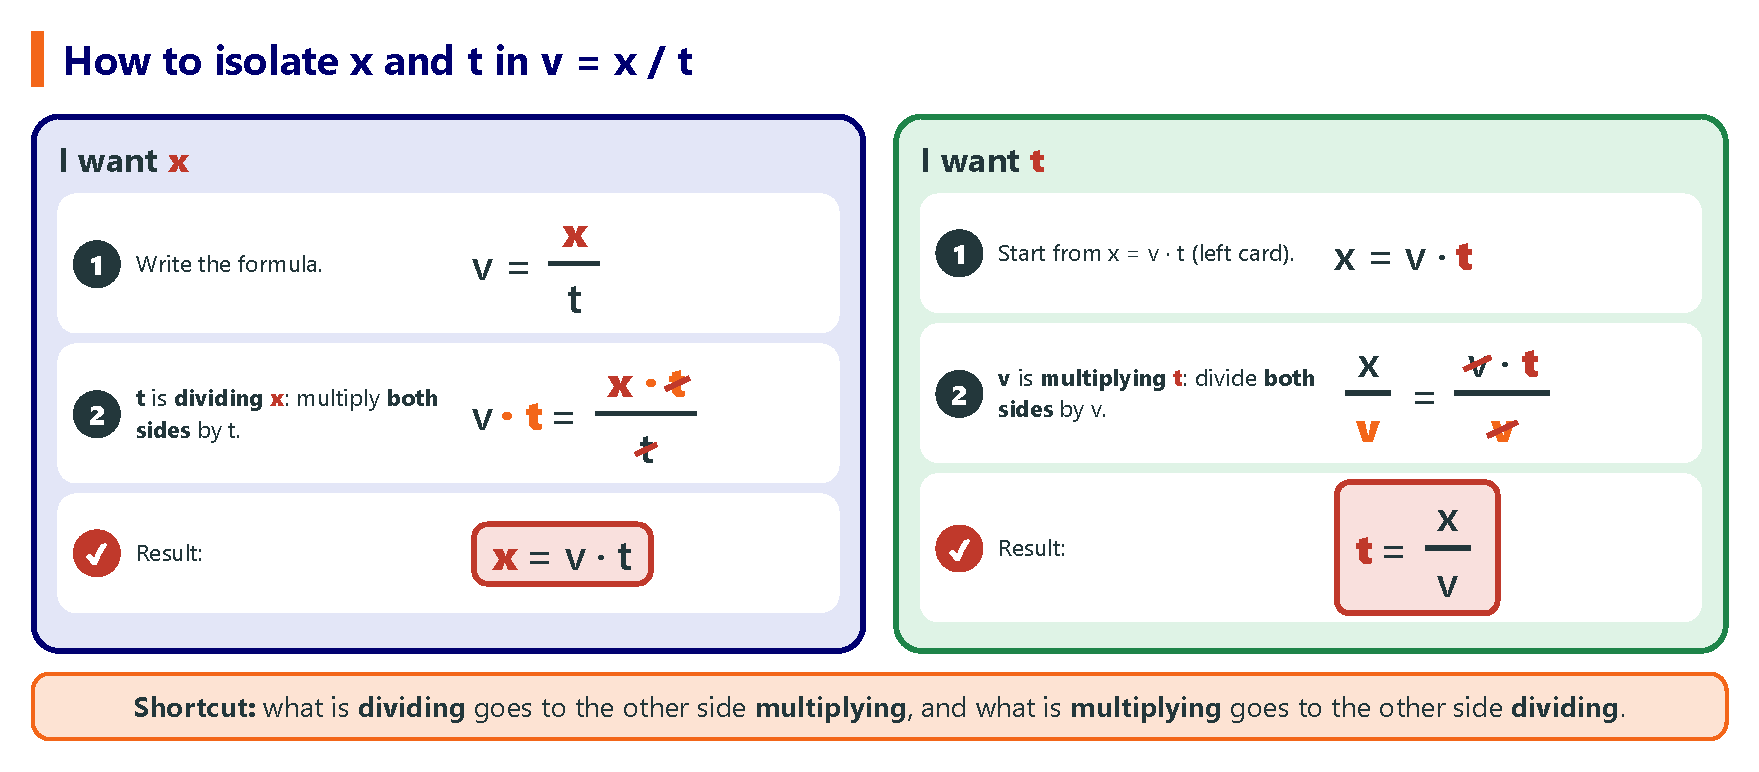
\includegraphics[width=\textwidth]{FigurasSVG/Unit_7_Motion/pdf/velocity_isolate.pdf}
    \caption{Isolating the position \(x\) and the time \(t\) in \(v = x/t\), step by step.}
    \label{fig:u7_velocity_isolate}
\end{figure}

\negsubro{Isolating the position \(x\)}:
\begin{enumerate}[label=\numberballmDarkTeal]
    \item We write the formula: \(v = \dfrac{x}{t}\).
    \item \(t\) is \textbf{dividing} \(x\), so we \textbf{multiply both sides} by \(t\): \(\;v \cdot t = \dfrac{x \cdot \cancelred{t}}{\cancelred{t}}\).
    \item \(t/t = 1\), so it cancels. We turn the equation round: \(\textcolor{red}{x = v \cdot t}\).
\end{enumerate}

\negsubro{Isolating the time \(t\)}:
\begin{enumerate}[label=\numberballmDarkTeal]
    \item We start from \(x = v \cdot t\) (the result above).
    \item \(v\) is \textbf{multiplying} \(t\), so we \textbf{divide both sides} by \(v\): \(\;\dfrac{x}{v} = \dfrac{\cancelred{v} \cdot t}{\cancelred{v}}\).
    \item \(v/v = 1\), so it cancels. We turn the equation round: \(\textcolor{red}{t = \dfrac{x}{v}}\).
\end{enumerate}

\begin{impt}
    The three versions of the same formula (with \(x_i = \qty{0}{\m}\) and \(t_i = \qty{0}{\s}\)):
    \begin{equation*}
        v = \dfrac{x}{t} \qquad\qquad x = v \cdot t \qquad\qquad t = \dfrac{x}{v}
    \end{equation*}
    \textbf{Shortcut}: what is \textbf{dividing} on one side goes to the other side \textbf{multiplying}, and what is \textbf{multiplying} goes to the other side \textbf{dividing}.
\end{impt}

\begin{example}
    \textbf{Calculating a position. A cyclist rides at a constant \qty{6}{\mps} for \qty{50}{\s}. Where is she at the end, if she started at the origin?}
    \begin{enumerate}[label=\numberballmDarkTeal]
        \item Data: \(v = \qty{6}{\mps}\), \(t = \qty{50}{\s}\), \(x_i = \qty{0}{\m}\). Unknown: \(\underline{x}\).
        \item Formula: \(v = \dfrac{x}{t}\). \(t\) is dividing, so it goes to the other side multiplying: \(x = v \cdot t\).
        \item \(x = \qty{6}{\mps} \cdot \qty{50}{\s} = \textcolor{red}{\qty{300}{\m}}\).
    \end{enumerate}
\end{example}

\begin{example}
    \textbf{Calculating a time. How long does a walker moving at a constant \qty{1.5}{\mps} take to walk \qty{1200}{\m}?}
    \begin{enumerate}[label=\numberballmDarkTeal]
        \item Data: \(v = \qty{1.5}{\mps}\), \(x = \qty{1200}{\m}\). Unknown: \(\underline{t}\).
        \item Formula: \(x = v \cdot t\). \(v\) is multiplying, so it goes to the other side dividing: \(t = \dfrac{x}{v}\).
        \item \(t = \dfrac{\qty{1200}{\m}}{\qty{1.5}{\mps}} = \textcolor{red}{\qty{800}{\s}}\) (about \qty{13.3}{\minute}).
    \end{enumerate}
\end{example}

\begin{exercise}
    Isolate the unknown and calculate (all the objects start at the origin and move in URM):
    \begin{enumerate}[label=\letraminuscula]
        \item The position of a car that travels at \qty{25}{\mps} for \qty{40}{\s}.
        \item The time a snail moving at \qty{0.002}{\mps} needs to travel \qty{1}{\m}.
        \item The time sound needs to travel \qty{1700}{\m} (\(v = \qty{340}{\mps}\)).
        \item The position of a train moving at \qty{30}{\mps} after \qty{2}{\minute} (change the time to seconds first).
    \end{enumerate}
    \begin{solu}
        \begin{enumerate}[label=\alph*)]
            \item \(x = v \cdot t = \qty{25}{\mps} \cdot \qty{40}{\s} = \qty{1000}{\m}\).
            \item \(t = \dfrac{x}{v} = \dfrac{\qty{1}{\m}}{\qty{0.002}{\mps}} = \qty{500}{\s}\).
            \item \(t = \dfrac{x}{v} = \dfrac{\qty{1700}{\m}}{\qty{340}{\mps}} = \qty{5}{\s}\).
            \item \(t = \qty{2}{\minute} = \qty{120}{\s}\); \(x = v \cdot t = \qty{30}{\mps} \cdot \qty{120}{\s} = \qty{3600}{\m}\).
        \end{enumerate}
    \end{solu}
\end{exercise}

\subsection{Position-time graphs in URM}

\begin{figure}[H]
    \centering
    % [FIGURA ORIGINAL] \includegraphics[width=\textwidth]{Unit_7/urm_graphs}
    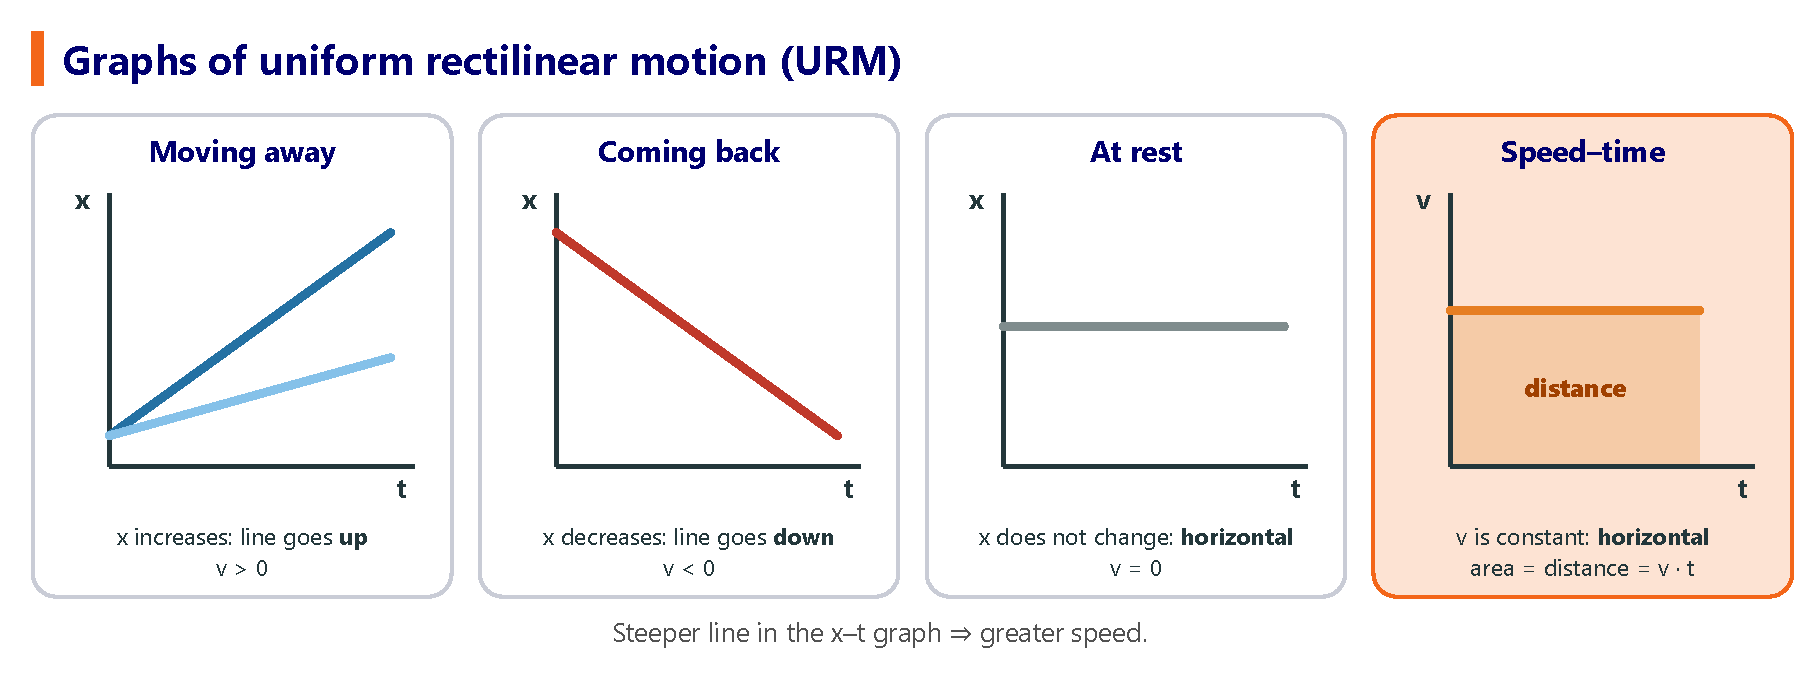
\includegraphics[width=\textwidth]{FigurasSVG/Unit_7_Motion/pdf/urm_graphs.pdf}
    \caption{Position-time and speed-time graphs of a URM.}
    \label{fig:u7_urm_graphs}
\end{figure}

\begin{itemize}
    \item If the position \textbf{increases} with time, the line goes up, and the object is moving away from the origin.
    \item If the position \textbf{decreases} with time, the line goes down, and the object is moving towards the origin (or past it, into negative positions).
    \item The graph of a URM is always a \textbf{straight line}. The more inclined the line, the greater the speed.
    \item If the line passes through the point \((0,0)\), the object was at the origin when we started studying its motion; if not, the object was already at another position.
\end{itemize}

\begin{impt}
    \negsubro{Reading two URM lines on the same graph}: when two position-time lines are drawn on the same axes, the point where they \textbf{cross} represents the moment and the position at which the two objects meet (they are, at that instant, at the same place).
\end{impt}

\begin{figure}[H]
    \centering
    % [FIGURA ORIGINAL] \includegraphics[width=0.95\textwidth]{Unit_7/meeting}
    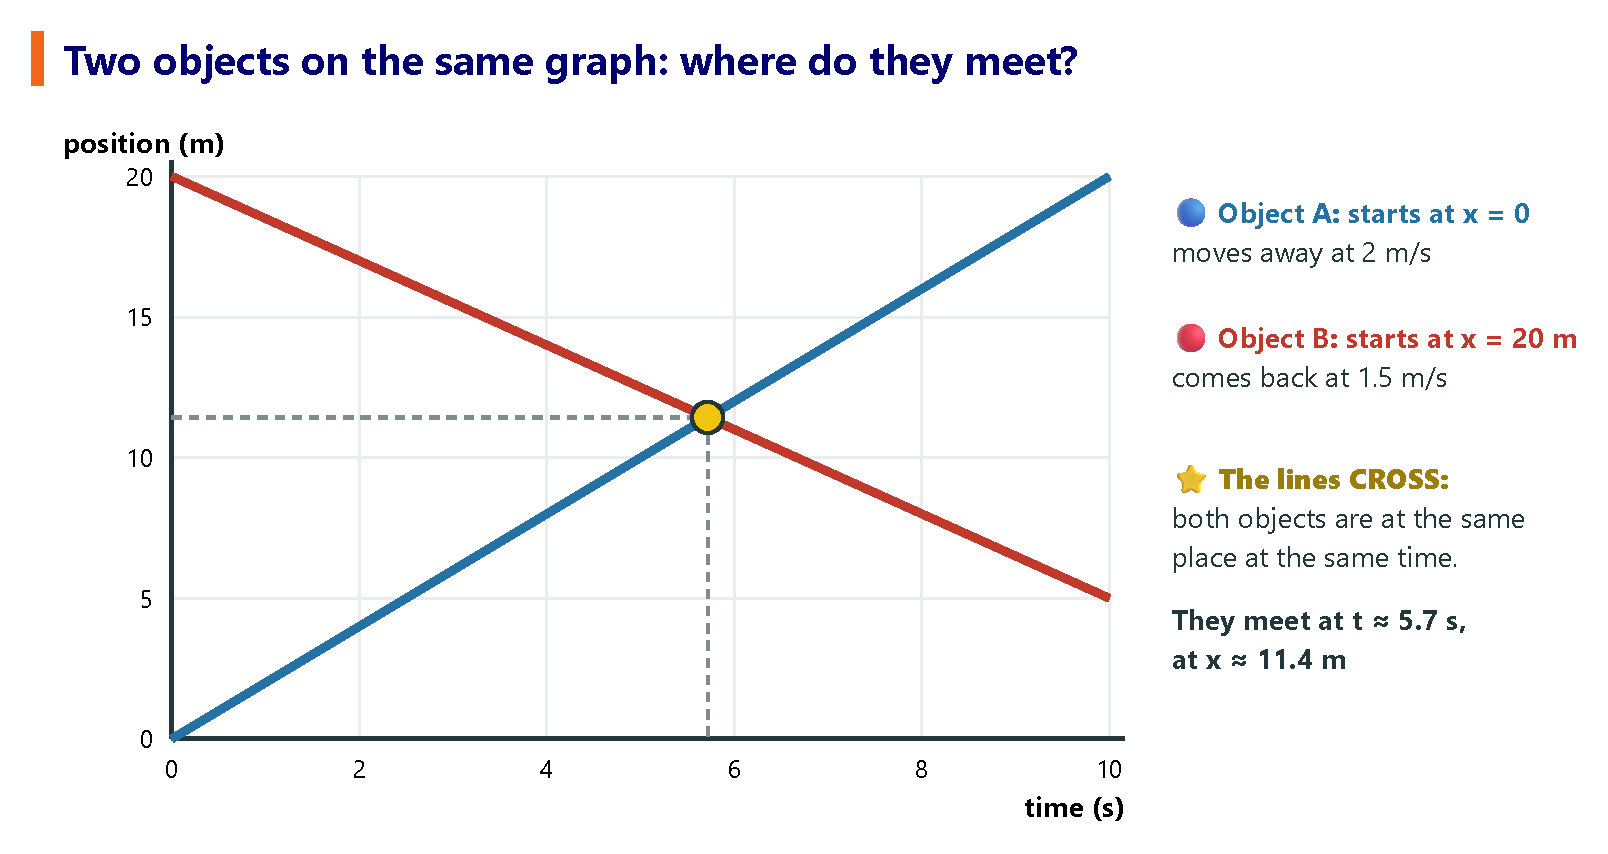
\includegraphics[width=0.95\textwidth]{FigurasSVG/Unit_7_Motion/pdf/meeting.pdf}
    \caption{When two position-time lines cross, the two objects are at the same place at the same time.}
    \label{fig:u7_meeting}
\end{figure}

\begin{example}
    \textbf{Two positions are recorded for a walker every second: at \(t=\qty{2}{\s}\), \(x=\qty{3}{\m}\); at \(t=\qty{6}{\s}\), \(x=\qty{11}{\m}\). Is the position-time graph increasing or decreasing? What does this tell us about the walker's direction?}

    Since \(x\) increases from \(\qty{3}{\m}\) to \(\qty{11}{\m}\) as \(t\) increases, the line on the position-time graph goes \textbf{up}: the walker is moving \textbf{away} from the origin. The speed can also be found from these two points: \(v = \dfrac{11-3}{6-2} = \qty{2}{\mps}\).
\end{example}

\begin{exercise}
    A position-time graph shows a straight horizontal line at \(x = \qty{12}{\m}\), from \(t=0\) to \(t=\qty{10}{\s}\).
    \begin{enumerate}[label=\letraminuscula]
        \item What is the object's speed?
        \item Is the object moving with respect to the chosen frame of reference?
    \end{enumerate}
    \begin{solu}
        \begin{enumerate}[label=\alph*)]
            \item Since the position does not change, \(v = \qty{0}{\mps}\).
            \item No: a horizontal line on a position-time graph means the object stays at the same position, so it is \textbf{at rest} with respect to this frame of reference.
        \end{enumerate}
    \end{solu}
\end{exercise}

\begin{exercise}
    The position-time graph of an object in URM is a straight line that passes through the origin \((0,0)\) and through the point \((t,x) = (\qty{5}{\s}, \qty{15}{\m})\).
    \begin{enumerate}[label=\letraminuscula]
        \item Was the object at the origin at \(t=0\)?
        \item Calculate its speed.
        \item Predict its position at \(t=\qty{8}{\s}\).
    \end{enumerate}
    \begin{solu}
        \begin{enumerate}[label=\alph*)]
            \item Yes: the line passes through \((0,0)\), so the object started at the origin.
            \item \(v = \dfrac{\qty{15}{\m} - 0}{\qty{5}{\s} - 0} = \qty{3}{\mps}\).
            \item \(x(8) = v \cdot t = \qty{3}{\mps} \cdot \qty{8}{\s} = \qty{24}{\m}\).
        \end{enumerate}
    \end{solu}
\end{exercise}

\begin{exercise}
    The position-time graph of a URM is shown below.
    \begin{center}
        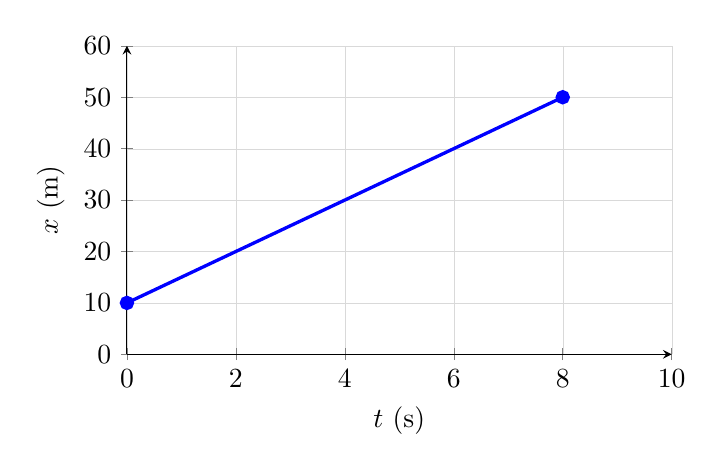
\begin{tikzpicture}
            \begin{axis}[width=8.5cm, height=5.5cm, grid=both, grid style={line width=.1pt, draw=gray!30},
                axis lines=left, xlabel={\(t\) (s)}, ylabel={\(x\) (m)}, xmin=0, xmax=10, ymin=0, ymax=60, xtick={0,2,...,10}, ytick={0,10,...,60}]
                \addplot[very thick, blue, mark=*] coordinates {(0,10) (8,50)};
            \end{axis}
        \end{tikzpicture}
    \end{center}
    \begin{enumerate}[label=\letraminuscula]
        \item What is the initial position \(x_i\) of the object?
        \item Calculate its velocity, using \(x_i\), \(x_f\), \(t_i\) and \(t_f\).
        \item Is the object moving away from the origin or towards it?
        \item Read on the graph the position at \(t = \qty{4}{\s}\), and check it with a calculation.
    \end{enumerate}
    \begin{solu}
        \begin{enumerate}[label=\alph*)]
            \item At \(t = \qty{0}{\s}\) the line starts at \(x_i = \qty{10}{\m}\): the object did not start at the origin.
            \item \(v = \dfrac{x_f - x_i}{t_f - t_i} = \dfrac{\qty{50}{\m} - \qty{10}{\m}}{\qty{8}{\s} - \qty{0}{\s}} = \qty{5}{\mps}\).
            \item The line goes up (\(v > 0\)): it is moving \textbf{away} from the origin.
            \item From the graph, \(x = \qty{30}{\m}\). Calculation: \(x = x_i + v \cdot t = \qty{10}{\m} + \qty{5}{\mps} \cdot \qty{4}{\s} = \qty{30}{\m}\).
        \end{enumerate}
    \end{solu}
\end{exercise}

\begin{exercise}
    The graph shows the position of a student walking along a straight corridor.
    \begin{center}
        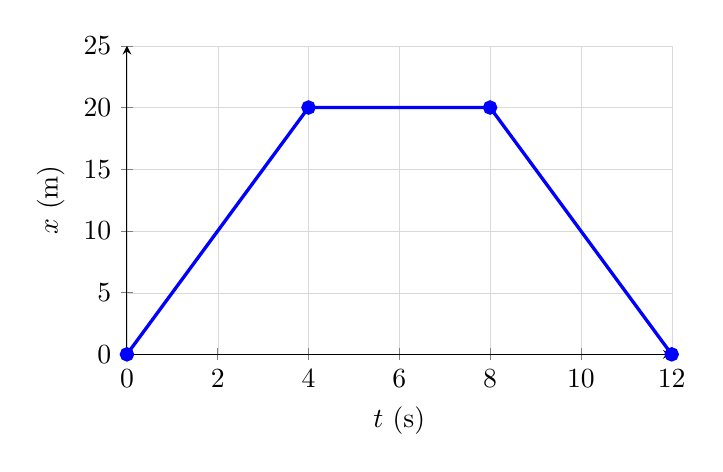
\begin{tikzpicture}
            \begin{axis}[width=8.5cm, height=5.5cm, grid=both, grid style={line width=.1pt, draw=gray!30},
                axis lines=left, xlabel={\(t\) (s)}, ylabel={\(x\) (m)}, xmin=0, xmax=12, ymin=0, ymax=25, xtick={0,2,...,12}, ytick={0,5,...,25}]
                \addplot[very thick, blue, mark=*] coordinates {(0,0) (4,20) (8,20) (12,0)};
            \end{axis}
        \end{tikzpicture}
    \end{center}
    \begin{enumerate}[label=\letraminuscula]
        \item Describe what the student does in each section: \(0\)--\(4\) s, \(4\)--\(8\) s and \(8\)--\(12\) s.
        \item Calculate the velocity in each section.
        \item Calculate the total distance travelled and the total displacement.
    \end{enumerate}
    \begin{solu}
        \begin{enumerate}[label=\alph*)]
            \item \(0\)--\(4\) s: moves away from the origin. \(4\)--\(8\) s: stays at \(x = \qty{20}{\m}\) (at rest). \(8\)--\(12\) s: comes back to the origin.
            \item \(v_1 = \dfrac{20 - 0}{4 - 0} = \qty{5}{\mps}\); \quad \(v_2 = \dfrac{20 - 20}{8 - 4} = \qty{0}{\mps}\); \quad \(v_3 = \dfrac{0 - 20}{12 - 8} = \qty{-5}{\mps}\).
            \item Distance travelled \(= \qty{20}{\m} + \qty{0}{\m} + \qty{20}{\m} = \qty{40}{\m}\). Displacement \(\Delta x = x_f - x_i = \qty{0}{\m} - \qty{0}{\m} = \qty{0}{\m}\) (he ends where he started).
        \end{enumerate}
    \end{solu}
\end{exercise}

\begin{exercise}
    The graph shows the positions of two cars, \(A\) and \(B\), moving along the same straight road.
    \begin{center}
        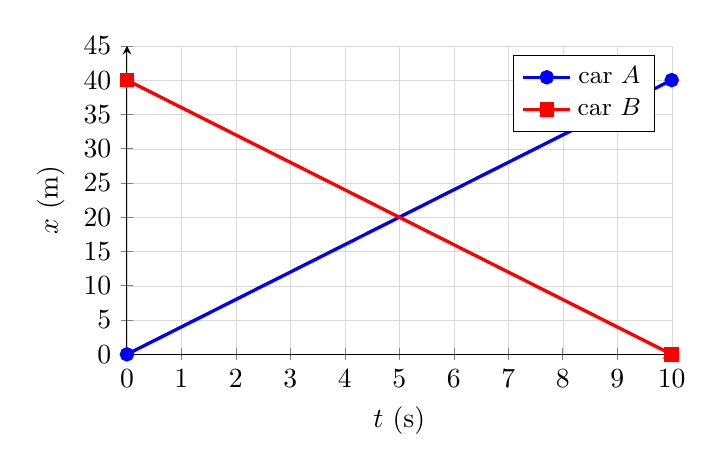
\begin{tikzpicture}
            \begin{axis}[width=8.5cm, height=5.5cm, grid=both, grid style={line width=.1pt, draw=gray!30},
                axis lines=left, xlabel={\(t\) (s)}, ylabel={\(x\) (m)}, xmin=0, xmax=10, ymin=0, ymax=45, xtick={0,1,...,10}, ytick={0,5,...,45}, legend pos=north east, legend style={font=\small}]
                \addplot[very thick, blue, mark=*] coordinates {(0,0) (10,40)};
                \addlegendentry{car \(A\)}
                \addplot[very thick, red, mark=square*] coordinates {(0,40) (10,0)};
                \addlegendentry{car \(B\)}
            \end{axis}
        \end{tikzpicture}
    \end{center}
    \begin{enumerate}[label=\letraminuscula]
        \item Calculate the velocity of each car. What does the sign of each velocity mean?
        \item At what time and in what position do the two cars meet?
    \end{enumerate}
    \begin{solu}
        \begin{enumerate}[label=\alph*)]
            \item \(v_A = \dfrac{40 - 0}{10 - 0} = \qty{4}{\mps}\) (positive: it moves away from the origin). \(v_B = \dfrac{0 - 40}{10 - 0} = \qty{-4}{\mps}\) (negative: it moves towards the origin).
            \item The lines cross at \(t = \qty{5}{\s}\) and \(x = \qty{20}{\m}\): the two cars meet there.
        \end{enumerate}
    \end{solu}
\end{exercise}

\begin{exercise}
    A toy car moves in URM. Its positions are recorded in this table:
    \begin{center}
        \begin{tabular}{lcccccc}
            \toprule
            \(t\) (s) & 0 & 1 & 2 & 3 & 4 & 5 \\
            \midrule
            \(x\) (m) & 0 & 3 & 6 & 9 & 12 & 15 \\
            \bottomrule
        \end{tabular}
    \end{center}
    \begin{enumerate}[label=\letraminuscula]
        \item Draw the position-time graph (\(t\) on the horizontal axis, \(x\) on the vertical axis).
        \item What shape does the graph have? Why?
        \item Calculate the velocity of the car.
    \end{enumerate}
    \begin{solu}
        \begin{enumerate}[label=\alph*)]
            \item The points \((0,0)\), \((1,3)\), \((2,6)\), \((3,9)\), \((4,12)\) and \((5,15)\) are joined with a straight line.
    \begin{center}
                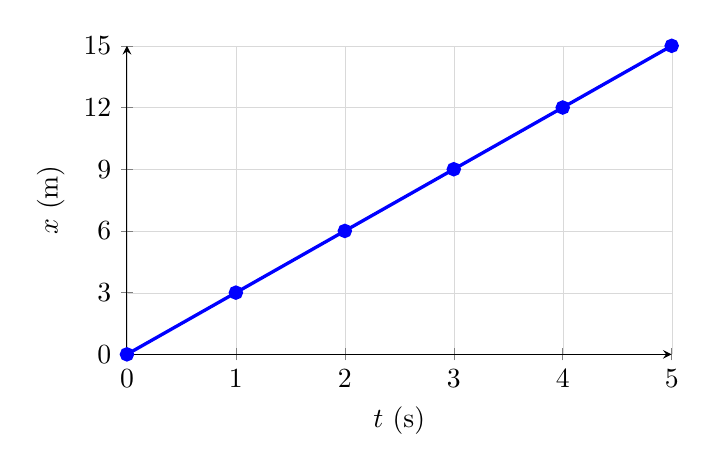
\begin{tikzpicture}
                    \begin{axis}[width=8.5cm, height=5.5cm, grid=both, grid style={line width=.1pt, draw=gray!30},
                        axis lines=left, xlabel={\(t\) (s)}, ylabel={\(x\) (m)}, xmin=0, xmax=5, ymin=0, ymax=15, xtick={0,1,...,5}, ytick={0,3,...,15}]
                        \addplot[very thick, blue, mark=*] coordinates {(0,0) (1,3) (2,6) (3,9) (4,12) (5,15)};
                    \end{axis}
                \end{tikzpicture}
            \end{center}
            \item A straight line going up through the origin, because the car covers the same distance (\qty{3}{\m}) every second: its velocity is constant.
            \item \(v = \dfrac{x_f - x_i}{t_f - t_i} = \dfrac{\qty{15}{\m} - \qty{0}{\m}}{\qty{5}{\s} - \qty{0}{\s}} = \qty{3}{\mps}\).
        \end{enumerate}
    \end{solu}
\end{exercise}

\subsection{Velocity in URM from a table or a graph}

To calculate the velocity of a URM, take any two points \(A\) and \(B\) from a table or graph. Point \(A\) is the \textbf{initial} one and point \(B\) the \textbf{final} one:
\begin{equation*}
    x_A = x_i \qquad t_A = t_i \qquad\qquad x_B = x_f \qquad t_B = t_f
\end{equation*}
So the formula is exactly the same formula of velocity that we already know:
\begin{equation*}
    v = \dfrac{x_B - x_A}{t_B - t_A} = \dfrac{x_f - x_i}{t_f - t_i} = \dfrac{\Delta x}{\Delta t}
\end{equation*}

\begin{example}
    \textbf{A point \(A\) is at \(x = \qty{10}{\m}\) when \(t = \qty{4}{\s}\); a point \(B\) is at \(x = \qty{30}{\m}\) when \(t = \qty{12}{\s}\). Find the velocity.} \\
    Point \(A\) is the initial one: \(x_i = \qty{10}{\m}\), \(t_i = \qty{4}{\s}\). Point \(B\) is the final one: \(x_f = \qty{30}{\m}\), \(t_f = \qty{12}{\s}\).
    \begin{equation*}
        v = \dfrac{\qty{30}{\m} - \qty{10}{\m}}{\qty{12}{\s} - \qty{4}{\s}} = \qty{2.5}{\mps}
    \end{equation*}
    A \textbf{positive} speed means the object is moving away from the origin.
\end{example}

\begin{impt}
    If, instead, the position \textbf{decreases} between the two points, the speed comes out \textbf{negative}. This means the object is moving towards the origin (or beyond it).
\end{impt}

\begin{exercise}
    A point \(A\) is at \(x = \qty{50}{\m}\) when \(t = \qty{5}{\s}\); a point \(B\) is at \(x = \qty{20}{\m}\) when \(t = \qty{15}{\s}\).
    \begin{enumerate}[label=\letraminuscula]
        \item Calculate the speed.
        \item What does the sign of the speed tell you about the direction of motion?
    \end{enumerate}
    \begin{solu}
        \begin{enumerate}[label=\alph*)]
            \item \(v = \dfrac{\qty{20}{\m} - \qty{50}{\m}}{\qty{15}{\s} - \qty{5}{\s}} = \qty{-3}{\mps}\).
            \item The speed is \textbf{negative}, so the object is moving towards the origin (its position decreases with time).
        \end{enumerate}
    \end{solu}
\end{exercise}

\begin{exercise}
    The table shows the position of a toy train every \qty{3}{\s}:
    \begin{center}
        \begin{tabular}{lcccc}
            \toprule
            Time (s) & 0 & 3 & 6 & 9 \\
            \midrule
            Position (m) & 2 & 14 & 26 & 38 \\
            \bottomrule
        \end{tabular}
    \end{center}
    \begin{enumerate}[label=\letraminuscula]
        \item Calculate the speed using the first two points in the table.
        \item Check, using another pair of points, that the motion is indeed a URM.
        \item Predict the train's position at \(t=\qty{12}{\s}\).
    \end{enumerate}
    \begin{solu}
        \begin{enumerate}[label=\alph*)]
            \item \(v = \dfrac{\qty{14}{\m} - \qty{2}{\m}}{\qty{3}{\s} - \qty{0}{\s}} = \qty{4}{\mps}\).
            \item Between \(t=6\) s and \(t=9\) s: \(v = \dfrac{38-26}{9-6} = \qty{4}{\mps}\), the same value, so the speed is constant: this confirms it is a URM.
            \item \(x(12) = x(0) + v \cdot t = \qty{2}{\m} + \qty{4}{\mps} \cdot \qty{12}{\s} = \qty{50}{\m}\).
        \end{enumerate}
    \end{solu}
\end{exercise}

\subsection{Velocity-time graphs in URM}

Since the velocity of a URM is constant, its velocity-time graph is always a \textbf{horizontal line}.

\begin{impt}
    \negsubro{Distance travelled from a speed-time graph}: the distance travelled equals the \textbf{area} between the speed-time line and the time axis. In a URM this area is a rectangle: \(\text{distance} = v \cdot t\), which is the same equation we already use to calculate the speed.
\end{impt}

\begin{example}
    \textbf{A cyclist moves at a constant \qty{4}{\mps} for \qty{15}{\s}. Find the distance travelled using the area under the speed-time graph.}

    The speed-time graph is a horizontal line at \(v = \qty{4}{\mps}\), between \(t=0\) and \(t=\qty{15}{\s}\). The area underneath is a rectangle:
    \begin{equation*}
        \text{distance} = v \cdot t = \qty{4}{\mps} \cdot \qty{15}{\s} = \qty{60}{\m}
    \end{equation*}
\end{example}

\begin{exercise}
    The table shows the position of a remote-controlled car every \qty{10}{\s}:
    \begin{center}
        \begin{tabular}{lcccc}
            \toprule
            Time (s) & 0 & 10 & 20 & 30 \\
            \midrule
            Position (m) & 10 & 30 & 30 & 0 \\
            \bottomrule
        \end{tabular}
    \end{center}
    \begin{enumerate}[label=\letraminuscula]
        \item Calculate the speed in each section of its journey.
        \item Calculate the average speed of the whole journey.
    \end{enumerate}
    \begin{solu}
        \begin{enumerate}[label=\alph*)]
            \item Section 1 (\(t=0\) to \(10\) s): \(v_1 = \dfrac{30-10}{10-0} = \qty{2}{\mps}\). \\
            Section 2 (\(t=10\) to \(20\) s): the position does not change, so \(v_2 = \qty{0}{\mps}\) (the car is at rest). \\
            Section 3 (\(t=20\) to \(30\) s): \(v_3 = \dfrac{0-30}{30-20} = \qty{-3}{\mps}\) (moving towards the origin).
            \item Total distance travelled \(= \qty{20}{\m} + \qty{0}{\m} + \qty{30}{\m} = \qty{50}{\m}\); total time \(= \qty{30}{\s}\). \\
            \(v_{\text{average}} = \dfrac{50}{30} \approx \qty{1.67}{\mps}\).
        \end{enumerate}
    \end{solu}
\end{exercise}

\begin{exercise}
    A cyclist passes the \qty{20}{\km} mark when the stopwatch is started, moving at a constant speed. She reaches the \qty{40}{\km} mark after \qty{25}{\minute}, stops to rest for \qty{20}{\minute}, and then travels the next \qty{20}{\km} in \qty{10}{\minute}, again at a constant speed.
    \begin{enumerate}[label=\letraminuscula]
        \item Calculate her speed in each of the three sections.
        \item Calculate her average speed for the whole journey.
    \end{enumerate}
    \begin{solu}
        \begin{enumerate}[label=\alph*)]
            \item Section 1: \(v_1 = \dfrac{40\qty{-20}{\km}}{25\qty{-0}{\minute}} = \qty{0.8}{\km\per\minute}\). \\
            Section 2 (resting): \(v_2 = \qty{0}{\km\per\minute}\). \\
            Section 3: \(v_3 = \dfrac{60\qty{-40}{\km}}{55\qty{-45}{\minute}} = \qty{2}{\km\per\minute}\).
            \item Total distance \(= \qty{40}{\km}\); total time \(= 25 + 20 + 10 = \qty{55}{\minute}\) (the rest is included). \\
            \(v_{\text{average}} = \dfrac{40}{55} \approx \qty{0.73}{\km\per\minute}\).
        \end{enumerate}
    \end{solu}
\end{exercise}

\begin{exercise}
    Two trains, \(A\) and \(B\), travel towards each other along the same straight track. Train \(A\) starts at position \(x=\qty{0}{\km}\) and moves at \(\qty{80}{\kmph}\). Train \(B\) starts, at the same instant, at position \(x=\qty{300}{\km}\) and moves at \(\qty{70}{\kmph}\) towards \(A\).
    \begin{enumerate}[label=\letraminuscula]
        \item Write the position of each train as a function of time, \(x_A(t)\) and \(x_B(t)\).
        \item Find the time and the position at which the two trains meet.
    \end{enumerate}
    \begin{solu}
        \begin{enumerate}[label=\alph*)]
            \item \(x_A(t) = 80 \cdot t\) (moving away from the origin). \\
            \(x_B(t) = 300 - 70 \cdot t\) (moving towards the origin).
            \item They meet when \(x_A(t) = x_B(t)\): \(80t = 300 - 70t \;\Rightarrow\; 150t = 300 \;\Rightarrow\; t = \qty{2}{\hour}\). \\
            Position: \(x_A(2) = 80 \cdot 2 = \qty{160}{\km}\) (checking: \(x_B(2) = 300 - 70\cdot 2 = \qty{160}{\km}\), the same). \\
            The trains meet after \qty{2}{\hour}, at \(x = \qty{160}{\km}\).
        \end{enumerate}
    \end{solu}
\end{exercise}

\begin{exercise}
    A scooter moves at a constant \qty{3}{\mps} for \qty{20}{\s}, then stops for \qty{10}{\s}, and finally moves at a constant \qty{6}{\mps} for \qty{5}{\s}.
    \begin{enumerate}[label=\letraminuscula]
        \item Describe the shape of the speed-time graph in each of the three stages.
        \item Calculate the distance travelled in each stage, using the area under the graph.
        \item Calculate the average speed for the whole journey.
    \end{enumerate}
    \begin{solu}
        \begin{enumerate}[label=\alph*)]
            \item Stage 1: horizontal line at \(v=\qty{3}{\mps}\). Stage 2: horizontal line at \(v=\qty{0}{\mps}\) (on the time axis). Stage 3: horizontal line at \(v=\qty{6}{\mps}\).
            \item Stage 1: \(d_1 = \qty{3}{\mps} \cdot \qty{20}{\s} = \qty{60}{\m}\). Stage 2: \(d_2 = \qty{0}{\m}\). Stage 3: \(d_3 = \qty{6}{\mps} \cdot \qty{5}{\s} = \qty{30}{\m}\).
            \item Total distance \(= 60 + 0 + 30 = \qty{90}{\m}\); total time \(= 20+10+5 = \qty{35}{\s}\). \\
            \(v_{\text{average}} = \dfrac{90}{35} \approx \qty{2.57}{\mps}\).
        \end{enumerate}
    \end{solu}
\end{exercise}

%----------------------------------------------------------------------------------------

\section{Acceleration}

The speed of a moving object almost never stays constant throughout a journey: it usually increases or decreases.

\begin{definition}[Acceleration]
    A quantity that measures the change in speed per unit of time.
    \begin{equation*}
        a = \dfrac{v_{\text{final}} - v_{\text{initial}}}{\text{time taken}}
    \end{equation*}
    In the SI, acceleration is measured in \unit{\mpss}.
\end{definition}

\begin{figure}[H]
    \centering
    % [FIGURA ORIGINAL] \includegraphics[width=\textwidth]{Unit_7/acceleration}
    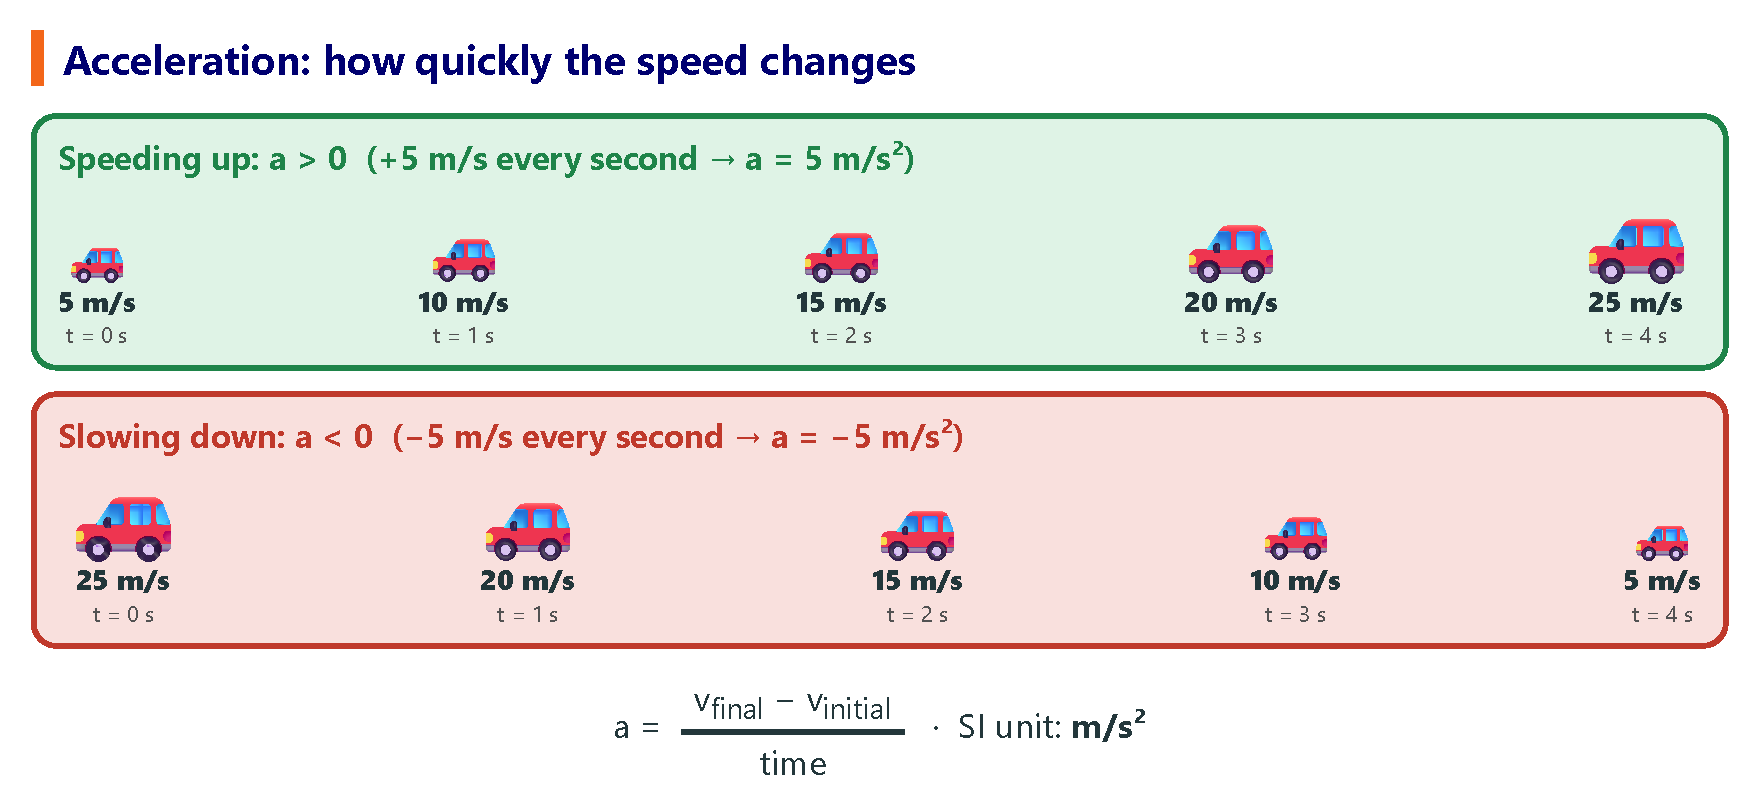
\includegraphics[width=\textwidth]{FigurasSVG/Unit_7_Motion/pdf/acceleration.pdf}
    \caption{Positive acceleration: the speed increases. Negative acceleration: the speed decreases.}
    \label{fig:u7_acceleration}
\end{figure}

\begin{itemize}
    \item If \(a > 0\) (\textbf{positive}), the object speeds up.
    \item If \(a < 0\) (\textbf{negative}), the object slows down.
\end{itemize}

\begin{example}
    \textbf{The speed of a car goes from \qty{5}{\mps} to \qty{25}{\mps} in four seconds. Calculate its acceleration.}
    \begin{equation*}
        a = \dfrac{\qty{25}{\mps} - \qty{5}{\mps}}{\qty{4}{\s}} = \dfrac{\qty{20}{\mps}}{\qty{4}{\s}} = \qty{5}{\mpss}
    \end{equation*}
\end{example}

\begin{exercise}
    A ball rolling at \qty{12}{\mps} decelerates uniformly and comes to a stop after \qty{6}{\s}.
    \begin{enumerate}[label=\letraminuscula]
        \item Calculate its acceleration.
        \item Is the sign of the acceleration what you expected? Explain.
    \end{enumerate}
    \begin{solu}
        \begin{enumerate}[label=\alph*)]
            \item \(a = \dfrac{0 - \qty{12}{\mps}}{\qty{6}{\s}} = \qty{-2}{\mpss}\).
            \item Yes: the acceleration is \textbf{negative} because the ball is slowing down (its speed decreases with time).
        \end{enumerate}
    \end{solu}
\end{exercise}

\begin{exercise}
    An object's speed changes from \(\qty{-4}{\mps}\) to \(\qty{-12}{\mps}\) in \qty{4}{\s} (a negative speed means it is moving towards the origin).
    \begin{enumerate}[label=\letraminuscula]
        \item Calculate the acceleration.
        \item Is the object speeding up or slowing down? Does this match the sign of the acceleration you found in (a)?
    \end{enumerate}
    \begin{solu}
        \begin{enumerate}[label=\alph*)]
            \item \(a = \dfrac{\qty{-12}{\mps} - (\qty{-4}{\mps})}{\qty{4}{\s}} = \dfrac{\qty{-8}{\mps}}{\qty{4}{\s}} = \qty{-2}{\mpss}\).
            \item The object is \textbf{speeding up} (its speed goes from \qty{4}{\mps} to \qty{12}{\mps} in absolute value), even though the acceleration is negative. This shows that the sign of the acceleration tells us the \textbf{direction} in which the speed is changing, not simply whether the object speeds up or slows down: here, both the speed and the acceleration point in the negative direction, so the object speeds up.
        \end{enumerate}
    \end{solu}
\end{exercise}

\subsection{Uniformly accelerated rectilinear motion (UARM)}

\begin{definition}[UARM]
    The motion of an object with a \textbf{straight} trajectory and a \textbf{constant} (non-zero) acceleration: its speed increases, or decreases, by the same amount every second.
\end{definition}

\begin{itemize}
    \item \negsubro{Speed-time graph}: always a straight line. An \textbf{increasing} line means positive acceleration; a \textbf{decreasing} line means negative acceleration. The steeper the line, the greater the (absolute value of the) acceleration.
    \item \negsubro{Distance travelled}: unlike in a URM, the distance travelled in each equal period of time is \textbf{not} the same in a UARM — it increases if \(a>0\), and decreases if \(a<0\).
\end{itemize}

\begin{impt}
    \negsubro{Distance travelled from a speed-time graph, in a UARM}: as in a URM, the distance travelled equals the \textbf{area} between the speed-time line and the time axis. When the object starts from rest (\(v_0 = 0\)), this area is a triangle, so:
    \begin{equation*}
        \text{distance} = \dfrac{v_{\text{final}} \cdot t}{2}
    \end{equation*}
\end{impt}

\begin{figure}[H]
    \centering
    % [FIGURA ORIGINAL] \includegraphics[width=\textwidth]{Unit_7/uarm_graphs}
    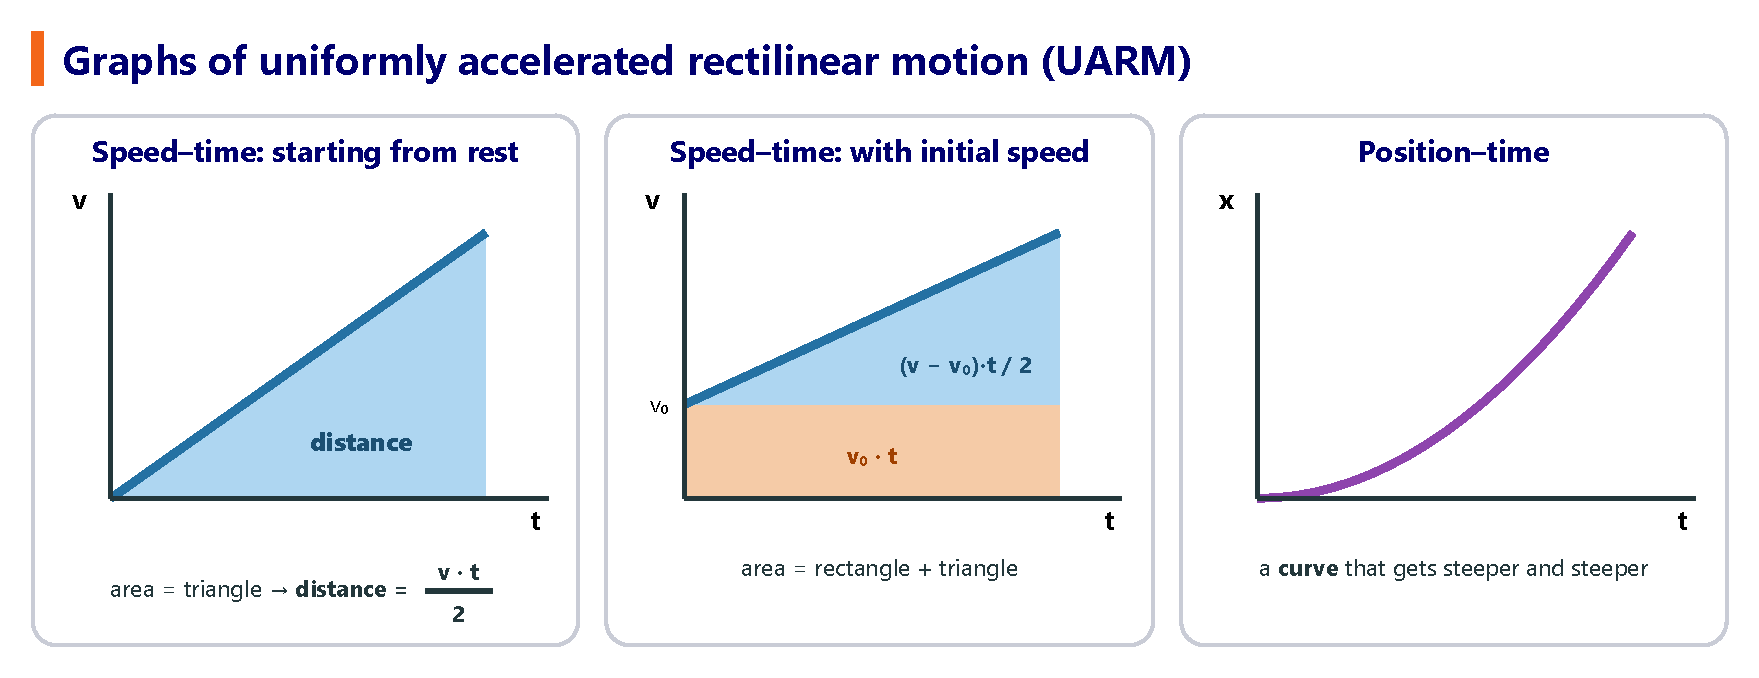
\includegraphics[width=\textwidth]{FigurasSVG/Unit_7_Motion/pdf/uarm_graphs.pdf}
    \caption{Graphs of a UARM: the area under the speed-time graph is the distance travelled.}
    \label{fig:u7_uarm_graphs}
\end{figure}

\begin{example}
    \textbf{A skateboarder starts from rest and speeds up to \qty{6}{\mps} in \qty{4}{\s}, with constant acceleration. Find the acceleration and the distance travelled.}
    \begin{equation*}
        a = \dfrac{\qty{6}{\mps} - 0}{\qty{4}{\s}} = \qty{1.5}{\mpss}
    \end{equation*}
    The speed-time graph is a triangle (a line from \((0,0)\) to \((4,6)\)), so:
    \begin{equation*}
        \text{distance} = \dfrac{v_{\text{final}} \cdot t}{2} = \dfrac{\qty{6}{\mps} \cdot \qty{4}{\s}}{2} = \qty{12}{\m}
    \end{equation*}
\end{example}

\begin{exercise}
    A car starts at \qty{5}{\mps} and accelerates uniformly to \qty{15}{\mps} in \qty{8}{\s}.
    \begin{enumerate}[label=\letraminuscula]
        \item Calculate its acceleration.
        \item The area under its speed-time graph is a trapezium: a rectangle of height \(v_0\) plus a triangle of height \(v_{\text{final}} - v_0\), both with base \(t\). Calculate the distance travelled.
    \end{enumerate}
    \begin{solu}
        \begin{enumerate}[label=\alph*)]
            \item \(a = \dfrac{\qty{15}{\mps} - \qty{5}{\mps}}{\qty{8}{\s}} = \qty{1.25}{\mpss}\).
            \item Rectangle: \(v_0 \cdot t = \qty{5}{\mps} \cdot \qty{8}{\s} = \qty{40}{\m}\). \\
            Triangle: \(\dfrac{(v_{\text{final}}-v_0)\cdot t}{2} = \dfrac{\qty{10}{\mps} \cdot \qty{8}{\s}}{2} = \qty{40}{\m}\). \\
            Total distance \(= 40 + 40 = \qty{80}{\m}\).
        \end{enumerate}
    \end{solu}
\end{exercise}

\begin{exercise}
    A cart starts from rest with a constant acceleration of \qty{2}{\mpss}.
    \begin{enumerate}[label=\letraminuscula]
        \item Complete a table with the speed every second, from \(t=0\) to \(t=4\) s.
        \item Calculate the distance travelled in those \qty{4}{\s}, using the triangle formula.
    \end{enumerate}
    \begin{solu}
        \begin{enumerate}[label=\alph*)]
            \item Since \(v = a \cdot t\):
            \begin{center}
                \begin{tabular}{cccccc}
                    \toprule
                    \(t\) (s) & 0 & 1 & 2 & 3 & 4 \\
                    \midrule
                    \(v\) (m/s) & 0 & 2 & 4 & 6 & 8 \\
                    \bottomrule
                \end{tabular}
            \end{center}
            \item \(\text{distance} = \dfrac{v_{\text{final}} \cdot t}{2} = \dfrac{\qty{8}{\mps} \cdot \qty{4}{\s}}{2} = \qty{16}{\m}\).
        \end{enumerate}
    \end{solu}
\end{exercise}

%\subsection{Free fall: a case of UARM}
%
%\begin{definition}[Free fall]
%    The motion of an object that falls, starting from rest, only under the effect of gravity, with no other force (such as air resistance) acting on it.
%\end{definition}
%
%\begin{figure}[H]
%    \centering
%    \includegraphics[width=0.95\textwidth]{Unit_7/free_fall}
%    \caption{Free fall: the speed increases by about \qty{10}{\mps} every second.}
%    \label{fig:u7_free_fall}
%\end{figure}
%
%\begin{impt}
%    Free fall is a \textbf{UARM} in the vertical direction. Near the Earth's surface, every falling object gains the same speed each second, regardless of its mass: the acceleration due to gravity is
%    \begin{equation*}
%        g \approx \qty{9.8}{\mpss} \quad (\text{often rounded to } \qty{10}{\mpss})
%    \end{equation*}
%    If air resistance is negligible, a heavier object does \textbf{not} fall faster than a lighter one.
%\end{impt}
%
%\begin{example}
%    \textbf{A stone is dropped from a bridge and falls for \qty{2}{\s} before hitting the water. Using \(g = \qty{10}{\mpss}\), find its speed on impact.}
%    \begin{equation*}
%        v = v_0 + g \cdot t = 0 + \qty{10}{\mpss} \cdot \qty{2}{\s} = \qty{20}{\mps}
%    \end{equation*}
%\end{example}
%
%\begin{exercise}
%    A ball is dropped from rest from a window and takes \qty{1.5}{\s} to reach the ground. Using \(g = \qty{10}{\mpss}\), calculate its speed just before hitting the ground.
%    \begin{solu}
%        \(v = v_0 + g \cdot t = 0 + \qty{10}{\mpss} \cdot \qty{1.5}{\s} = \qty{15}{\mps}\).
%    \end{solu}
%\end{exercise}
%
%\begin{exercise}
%    A motorbike starts from rest and accelerates at \qty{8}{\mpss} for the first five seconds.
%    \begin{enumerate}[label=\letraminuscula]
%        \item Make a table with the speed every second, from \(t=0\) to \(t=5\) s.
%    \end{enumerate}
%    \begin{solu}
%        Since \(v = v_0 + a \cdot t\), with \(v_0 = 0\) and \(a = \qty{8}{\mpss}\):
%        \begin{center}
%            \begin{tabular}{ccccccc}
%                \toprule
%                \(t\) (s) & 0 & 1 & 2 & 3 & 4 & 5 \\
%                \midrule
%                \(v\) (m/s) & 0 & 8 & 16 & 24 & 32 & 40 \\
%                \bottomrule
%            \end{tabular}
%        \end{center}
%    \end{solu}
%\end{exercise}
%
%\begin{exercise}
%    A car travelling at \qty{90}{\kmph} brakes and comes to a stop in \qty{10}{\s}.
%    \begin{enumerate}[label=\letraminuscula]
%        \item What was its acceleration?
%    \end{enumerate}
%    \begin{solu}
%        First convert the speed: \(\qty{90}{\kmph} = \qty{25}{\mps}\). \\
%        \(a = \dfrac{v_{\text{final}} - v_{\text{initial}}}{t} = \dfrac{0 - \qty{25}{\mps}}{\qty{10}{\s}} = \qty{-2.5}{\mpss}\) (negative, since the car slows down).
%    \end{solu}
%\end{exercise}
%
%\begin{exercise}
%    A cyclist moving at \qty{4}{\mps} accelerates uniformly at \qty{0.5}{\mpss} for \qty{6}{\s}.
%    \begin{enumerate}[label=\letraminuscula]
%        \item Calculate her final speed.
%        \item Sketch, in words, the shape of her speed-time graph and the shape of her distance-time graph (increasing/decreasing, straight/curved).
%    \end{enumerate}
%    \begin{solu}
%        \begin{enumerate}[label=\alph*)]
%            \item \(v_{\text{final}} = v_{\text{initial}} + a \cdot t = \qty{4}{\mps} + \qty{0.5}{\mpss} \cdot \qty{6}{\s} = \qty{7}{\mps}\).
%            \item The speed-time graph is a \textbf{straight, increasing} line (constant positive acceleration), starting at \(v=\qty{4}{\mps}\) instead of at zero. The position-time graph is \textbf{curved}, becoming steeper and steeper, because the speed (and therefore the distance covered per second) keeps increasing.
%        \end{enumerate}
%    \end{solu}
%\end{exercise}
%
%\begin{exercise}
%    A stone is dropped from rest and hits the ground after \qty{3}{\s}. Using \(g=\qty{10}{\mpss}\):
%    \begin{enumerate}[label=\letraminuscula]
%        \item Calculate its speed on impact.
%        \item Calculate the height from which it was dropped, using the triangle formula for the distance travelled.
%    \end{enumerate}
%    \begin{solu}
%        \begin{enumerate}[label=\alph*)]
%            \item \(v = v_0 + g \cdot t = 0 + \qty{10}{\mpss} \cdot \qty{3}{\s} = \qty{30}{\mps}\).
%            \item \(\text{height} = \dfrac{v_{\text{final}} \cdot t}{2} = \dfrac{\qty{30}{\mps} \cdot \qty{3}{\s}}{2} = \qty{45}{\m}\).
%        \end{enumerate}
%    \end{solu}
%\end{exercise}
%
%%----------------------------------------------------------------------------------------
%
%\section{Uniform circular motion (UCM)}
%
%\begin{definition}[Uniform circular motion (UCM)]
%    The motion of an object whose trajectory is a \textbf{circumference} and whose speed is \textbf{constant}.
%\end{definition}
%
%A UCM is a \textbf{periodic} motion, since it repeats at regular intervals of time.
%
%\begin{itemize}
%    \item \negsubro{Period}, \(T\): the time it takes the object to complete one full rotation.
%    \item \negsubro{Frequency}, \(f\): the number of rotations completed in a certain time; it is the inverse of the period. The greater the period, the lower the frequency.
%    \begin{equation*}
%        f = \dfrac{1}{T}
%    \end{equation*}
%\end{itemize}
%
%\begin{example}
%    The hour hand of a clock completes 1 rotation every 12 hours; the minute hand, 1 rotation every hour; the second hand, 1 rotation every minute. The hour hand has the \textbf{longest} period and the \textbf{lowest} frequency of the three.
%\end{example}
%
%\begin{example}
%    \textbf{The Earth rotates on its axis once a day. A point on the Equator (circumference length \qty{40077}{\km}) and a point on the Arctic Circle (circumference length \qty{15996}{\km}) both complete one rotation a day. Compare their periods, frequencies and speeds.}
%
%    Both points have the \textbf{same period} (\(T = \qty{24}{\hour}\)) and the \textbf{same frequency}, since they both complete one rotation per day. However, their \textbf{speeds} are different, because they travel different distances (different circumference lengths) in the same time:
%    \begin{equation*}
%        v_{\text{Equator}} = \dfrac{\qty{40077}{\km}}{\qty{24}{\hour}} \approx \qty{1670}{\kmph}
%        \qquad
%        v_{\text{Arctic Circle}} = \dfrac{\qty{15996}{\km}}{\qty{24}{\hour}} \approx \qty{666.5}{\kmph}
%    \end{equation*}
%\end{example}
%
%\begin{exercise}
%    Order the hour hand, minute hand and second hand of a clock by their period, from shortest to longest.
%    \begin{solu}
%        Second hand (\(T = \qty{1}{\minute}\)) \(<\) minute hand (\(T = \qty{1}{\hour}\)) \(<\) hour hand (\(T = \qty{12}{\hour}\)).
%    \end{solu}
%\end{exercise}
%
%\begin{exercise}
%    A fan blade completes 300 rotations per minute.
%    \begin{enumerate}[label=\letraminuscula]
%        \item Calculate its frequency, in \unit{\hertz}.
%        \item Calculate its period.
%    \end{enumerate}
%    \begin{solu}
%        \begin{enumerate}[label=\alph*)]
%            \item \(f = \dfrac{300 \text{ rotations}}{\qty{60}{\s}} = \qty{5}{\hertz}\).
%            \item \(T = \dfrac{1}{f} = \dfrac{1}{\qty{5}{\hertz}} = \qty{0.2}{\s}\).
%        \end{enumerate}
%    \end{solu}
%\end{exercise}
%
%\begin{exercise}
%    Wheel \(A\) has a period of \qty{0.5}{\s}. Wheel \(B\) completes 4 rotations every \qty{3}{\s}.
%    \begin{enumerate}[label=\letraminuscula]
%        \item Calculate the frequency of each wheel.
%        \item Which wheel is rotating faster?
%    \end{enumerate}
%    \begin{solu}
%        \begin{enumerate}[label=\alph*)]
%            \item \(f_A = \dfrac{1}{T_A} = \dfrac{1}{\qty{0.5}{\s}} = \qty{2}{\hertz}\). \\
%            \(f_B = \dfrac{4 \text{ rotations}}{\qty{3}{\s}} \approx \qty{1.33}{\hertz}\).
%            \item Since \(f_A > f_B\), \textbf{wheel \(A\)} completes more rotations per second, so it is rotating faster.
%        \end{enumerate}
%    \end{solu}
%\end{exercise}
%
%\subsection{Linear speed in UCM}
%
%\begin{definition}[Linear (tangential) speed in UCM]
%    In one period, an object in UCM travels a distance equal to the circumference length, \(2\pi r\), where \(r\) is the radius of the circular trajectory. Its (constant) linear speed is therefore:
%    \begin{equation*}
%        v = \dfrac{2\pi r}{T} = 2\pi r \cdot f
%    \end{equation*}
%\end{definition}
%
%\begin{figure}[H]
%    \centering
%    \includegraphics[width=\textwidth]{Unit_7/ucm}
%    \caption{Uniform circular motion: period, frequency and linear speed.}
%    \label{fig:u7_ucm}
%\end{figure}
%
%\begin{example}
%    \textbf{A carousel horse moves in a circle of radius \qty{4}{\m}, completing one turn every \qty{8}{\s}. Calculate its linear speed.}
%    \begin{equation*}
%        v = \dfrac{2\pi \cdot \qty{4}{\m}}{\qty{8}{\s}} \approx \qty{3.14}{\mps}
%    \end{equation*}
%\end{example}
%
%\begin{exercise}
%    A point on the rim of a bicycle wheel of radius \qty{0.35}{\m} completes 2 rotations per second.
%    \begin{enumerate}[label=\letraminuscula]
%        \item Calculate the period of its motion.
%        \item Calculate its linear speed.
%    \end{enumerate}
%    \begin{solu}
%        \begin{enumerate}[label=\alph*)]
%            \item \(T = \dfrac{1}{f} = \dfrac{1}{\qty{2}{\hertz}} = \qty{0.5}{\s}\).
%            \item \(v = 2\pi r \cdot f = 2\pi \cdot \qty{0.35}{\m} \cdot \qty{2}{\hertz} \approx \qty{4.4}{\mps}\).
%        \end{enumerate}
%    \end{solu}
%\end{exercise}
%
%\begin{exercise}
%    A satellite orbits the Earth in a circle of radius \qty{7000}{\km}, completing one orbit every \qty{2}{\hour}.
%    \begin{enumerate}[label=\letraminuscula]
%        \item Calculate its linear speed, in \unit{\kmph}.
%    \end{enumerate}
%    \begin{solu}
%        \(v = \dfrac{2\pi r}{T} = \dfrac{2\pi \cdot \qty{7000}{\km}}{\qty{2}{\hour}} \approx \qty{21991}{\kmph}\).
%    \end{solu}
%\end{exercise}
%
%\begin{exercise}
%    A point on a spinning disc of radius \qty{0.2}{\m} has a linear speed of \qty{4}{\mps}.
%    \begin{enumerate}[label=\letraminuscula]
%        \item Calculate its period.
%        \item Calculate its frequency.
%    \end{enumerate}
%    \begin{solu}
%        \begin{enumerate}[label=\alph*)]
%            \item From \(v = \dfrac{2\pi r}{T}\), we get \(T = \dfrac{2\pi r}{v} = \dfrac{2\pi \cdot \qty{0.2}{\m}}{\qty{4}{\mps}} \approx \qty{0.31}{\s}\).
%            \item \(f = \dfrac{1}{T} \approx \dfrac{1}{\qty{0.31}{\s}} \approx \qty{3.18}{\hertz}\).
%        \end{enumerate}
%    \end{solu}
%\end{exercise}

%----------------------------------------------------------------------------------------

\section*{Summary}

\begin{itemize}
    \item \textbf{Motion is relative} to the chosen frame of reference. Key quantities: position (\(x\)), trajectory, distance travelled and displacement.
    \item \textbf{Speed} \(= \) distance / time (SI unit: \unit{\mps}). Average speed uses the whole journey; instantaneous speed is read at one moment.
    \item \textbf{URM}: constant speed, straight trajectory; position-time graph is a straight line; speed-time graph is a horizontal line; distance = area under the speed-time graph.
    \item \textbf{Acceleration} \(=\) change in speed / time (SI unit: \unit{\mpss}). \textbf{UARM}: constant acceleration, straight trajectory; the distance travelled per equal time interval changes; distance = area under the speed-time graph (a triangle, if starting from rest).
    \item \textbf{Free fall} is a UARM with \(a = g \approx \qty{9.8}{\mpss}\), the same for every object regardless of its mass (if air resistance is negligible).
    \item \textbf{UCM}: circular trajectory, constant speed; described by the period \(T\) (time per rotation) and the frequency \(f = 1/T\); linear speed \(v = 2\pi r / T\).
\end{itemize}

\section{Vocabulary}

\begin{vocabulary}[Frame of reference]
    A fixed point, or set of points, used to describe the position and motion of a body. \newline
    \textbf{Translation to Spanish}: Sistema de referencia
\end{vocabulary}

\begin{vocabulary}[Trajectory]
    The line followed by a moving object. \newline
    \textbf{Translation to Spanish}: Trayectoria
\end{vocabulary}

\begin{vocabulary}[Displacement]
    The shortest distance between the initial and final position of a moving object. \newline
    \textbf{Translation to Spanish}: Desplazamiento
\end{vocabulary}

\begin{vocabulary}[Speed]
    A quantity that measures how fast an object moves; distance travelled per unit of time. \newline
    \textbf{Translation to Spanish}: Rapidez / velocidad
\end{vocabulary}

\begin{vocabulary}[Acceleration]
    A quantity that measures the change in speed per unit of time. \newline
    \textbf{Translation to Spanish}: Aceleración
\end{vocabulary}

\begin{vocabulary}[Uniform rectilinear motion]
    Motion with a straight trajectory and constant speed. \newline
    \textbf{Translation to Spanish}: Movimiento rectilíneo uniforme
\end{vocabulary}

\begin{vocabulary}[Uniform circular motion]
    Motion with a circular trajectory and constant speed. \newline
    \textbf{Translation to Spanish}: Movimiento circular uniforme
\end{vocabulary}

\begin{vocabulary}[Period]
    The time an object takes to complete one full rotation, in a periodic motion. \newline
    \textbf{Translation to Spanish}: Periodo
\end{vocabulary}

\begin{vocabulary}[Frequency]
    The number of rotations completed per unit of time. \newline
    \textbf{Translation to Spanish}: Frecuencia
\end{vocabulary}

\begin{vocabulary}[Free fall]
    The motion of an object falling from rest under the effect of gravity alone. \newline
    \textbf{Translation to Spanish}: Caída libre
\end{vocabulary}
